\onehalfspacing

\section{Lösungsansatz}

Bei der prototypischen Lösung steht im Zentrum dieser Arbeit die Wissensdatenbank \textit{Wikidata}\footnote{URL: \url{https://www.wikidata.org/wiki/Wikidata:Main_Page} (letzter Zugriff am 20.05.2022).} als offener Forschungsdatenmanagement-Service. Bei Wikidata handelt sich ursprünglich um ein offenes dankenbankbasiertes Angebot von Wikimedia für strukturierte Daten im Wiki*versum, das das Konzept von Linked Open Data umsetzt. Damit ist es flexibel und sprachenunabhängig einsetzbar, wodurch es als Modell auch für Forschungsdatenmanagement in der akademischen Wissenschaft interessant wird. Tatsächlich wird dieser Weg im Rahmen von NFDI gegenwärtig bestritten. Das \textit{Open Science Lab} am ,,Leibniz-Informationszentrum Technik und Naturwissenschaften und Universitätsbibliothek''\footnote{URL: \url{https://www.tib.eu/de/} (letzer Zugriff am 20.05.2022).} hat für das Konsortium \textit{NFDI4Culture}\footnote{URL: \url{https://nfdi4culture.de/index.html} (letzter Zugriff am 20.05.2022).} Wikidata und insbesondere die zugrunde liegende Software \textit{Wikibase}\footnote{URL: \url{https://wikibase.consulting/what-is-wikibase/} (letzter Zugriff am 20.05.2022).} auf die Einsetzbarkeit für ein Forschungsdatenmanagement von Kulturdaten hin evaluiert. Erste Ergebnisse wurden im März 2022 auf dem TIB-Blog veröffentlicht.\footnote{Siehe Lozana Rossenova (2022): Examining Wikidata and Wikibase in the context of research data management applications, veröffentlicht am 16.03.2022 auf dem TIB-Blog, URL: \url{https://blogs.tib.eu/wp/tib/2022/03/16/examining-wikidata-and-wikibase-in-the-context-of-research-data-management-applications/}.} Parallel führt das NFDI4Culture-Konsortium selbst die Workshop-Reihe ,,Wikibase'' durch.\footnote{URI: \url{https://nfdi4culture.de/resource/E2261/about.html}.} 

Auch im Kontext historischer Forschung kommt Wikidata bereits zum Einsatz. Das Online-Portal ,,Archivführer. Deutsche Kolonialgeschichte'' nutzt Wikidata als strukturierte Datenbasis für in Zusammenhang mit dem Thema ,,Deutsche Kolonien und Schutzgebiete'' stehende Forschungsdaten.\footnote{Das Projekt wurde 2017 an der Fachhochschule Potsdam initiiert und ist vom Auswärtigen Amt gefördert worden, URL: \url{https://archivfuehrer-kolonialzeit.de/} (letzter Zugriff am 20.05.2022).} Das Portal führt lediglich die Wikidata-Daten für die Datenpräsentation zusammen und ermöglicht einen multiperpektivischen Zugang zu den Daten.\footnote{Zum Beispiel Georeferenzierung der Orte anhand historischen Kartenmaterials, URL: \url{https://archivfuehrer-kolonialzeit.de/map} (letzter Zugriff am 20.05.2022).} Die Besonderheit ist, dass die Datenbereitstellung durch Wikidata ermöglicht, über die Projektlaufzeit hinaus Daten von jeder/jedem erweitern zu lassen sowie diese in gänzlich anderen Kontexten zu verwenden. Darüber hinaus verfolgt das Projekt das Ziel, die Daten mit der ,,kolonialen Vergangenheiten anderer Ländern''\footnote{URL: \url{https://archivfuehrer-kolonialzeit.de/about} (letzter Zugriff am 20.05.2022).} zu verknüpfen und auf diese Weise das Forschungsfeld zum Deutschen Kolonialismus anschlussfähig an die Forschung zum Europäischen Kolonialismus zu machen. Die Zusammenarbeit und der kollaborative Austausch dazu erfolgen ebenfalls global in Wikidata mit dem ,,Wikidata:WikiProject European Colonialism''.\footnote{URL: \url{Wikidata:WikiProject European Colonialism} (letzter Zugriff am 20.05.2022).} Das internationale Projekt ,,European Holocaust Research Infrastructure'' (EHRI), welches im Rahmen der Open Science-Strategie von der Europäischen Kommission seit 2017 gefördert wird\footnote{Im EU-Programm ,,Horizon Europe'', das bis 2027 läuft, URL: \url{https://ec.europa.eu/info/research-and-innovation/funding/funding-opportunities/funding-programmes-and-open-calls/horizon-europe_en}. Projektwebsite von EHRI, URL: \url{https://www.ehri-project.eu/} (alle letzter Zugriff am 20.05.2022).} nutzt Wikidata als zentrales Verzeichnis zur Erstellung einer Liste von Ghettos aus der Zeit des Holocausts.\footnote{Nancy Cooey (2018): Using Wikidata to build an authority list of Holocaust-era ghettos, veröffentlicht am 12.02.2018 auf dem EHRI Document Blog, URL: \url{https://blog.ehri-project.eu/2018/02/12/using-wikidata/\#Selecting\_Wikidata\_as\_a\_Tool} (letzter Zugriff am 20.05.2022).} Ziel ist, Daten aus verschiedenen Enzyklopädien, die bisher isoliert waren, in Wikidata erstmals zusammenzuführen und zu verknüpfen.\footnote{Vgl. ebd. Zentrale Enzyklopädien sind ,,The Yad Vashem Encyclopedia of the Ghettos During the Holocaust'' von Yad Vashem (Israel) und ,,USHMM Encyclopedia of Camps and Ghettos'' des United States Holocaust Memorial Museum (USA).}

Grundsätzlich ist bei der Implementierung des offenen Forschungsdatenmanagements mit Wikidata ist zu beachten, dass hier das Konzept von Linked (Open) Data umgesetzt wird, bei dem es sich, wie in Kapitel 2.2.2 bereits erläutert wurde, um einen wesentlichen Baustein des \textit{Semantic Web} handelt. Damit erfolgt offenes FDM in der höchsten Open Data-Stufe (= 5 Sterne). Vorteil ist, dass die Stärken dieses Konzepts, welche vor allem in der Verknüpfung und Vernetzung von Daten liegen, für das Forschungsdatenmanagement ausgenutzt werden können. Nachteilig ist, dass dieser Ansatz voraussetzungsreicher als andere Lösungen ist, da zum einen Kenntnisse der allgemeinen Technologien von Linked Data Web wie RDF (Resource Description Framework), JSON-LD (JavaScript Object Notation for Linked Data) oder URI (Uniform Ressource Identifier)\footnote{Im Rahmen dieser Arbeit können diese Technologien nicht detailliert vorgestellt werden, daher wird zur Vertiefung auf die Grundlagenliteratur verwiesen. Siehe zum Beispiel Malte Rehbein: Ontologien, in: Fotis Jannidis, Hubertus Kohle, Malte Rehbein (Hrsg.), Digital Humanities, 2017, doi:10.1007/978-3-476-05446-3\_11; Christian Stein: Linked Open Data – Wie das Web zur Semantik kam, in: Bibliothek Forschung und Praxis (Hrsg.), Band 38, Nr. 3, 2014, S. 447-455, doi:10.1515/bfp-2014-0055; Patrick Danowski, Adrian Pohl: (Open) Linked Data in Bibliotheken, Berlin, Boston, 2013, doi:10.1515/9783110278736; Gradmann, Steffen Hennicke, Marlies Olensky: Linked Data, in: Digitale Dienste für die Wissenschaft (Hrsg.), 2012, S. 18-22, doi.org/10.18452/6627;  } und zum anderen Kenntnisse des spezifische Metadatenschemas bzw. der Onotologie zugrunde liegenden Software Wikibase von Wikidata.\footnote{Siehe Mediawiki (2022): Wikibase/DataModel, URL:\url{https://www.mediawiki.org/wiki/Wikibase/DataModel} (letzter Zugriff am 22.05.2022).} für die Umsetzung benötigt werden.

\section{Erhebung}

\begin{quote}
    [...] Dass dieses methodisches Vorgehen auch transparent und nachvollziehbar ist.\footnote{B4\_Transkript, Pos. 67.}
\end{quote}

Datenerhebung in der empirischen historischen Forschung geht mit historischer Quellenanalyse und Quellenkritik einher.\footnote{Vgl. W. H. Schröder: Historische Sozialforschung: Forschungsstrategie - Infrastruktur - Auswahlbibliographie.
Historical Social Research, in: Supplement (Hrsg.) 1988, Nr. 1, S. 1-109, hier S. 15ff., URN: \url{https://nbn-resolving.org/urn:nbn:de:0168-ssoar-286038}
} Anders als in der naturwissenschaftlichen Datenerhebung, wo anhand von Experimenten, Beobachtungen, Simulationen oder Messungen, Daten in Echtzeit gewonnen werden und dementsprechend die Erhebungsmethoden an den Forschungsfragen angepasst werden können, ist die Vorgehensweise bei den geschichtswissenschaftlichen Disziplinen maßgeblich von der Überlieferungstruktur und der Quellensituation abhängig.\footnote{Was zu einem ,,Quellenproblem'' führen kann, siehe dazu ebd. S. 19f.} Informationen zur Erhebung sind also essentiell, um Forschungsdaten im Sinne einer Datenkritik kontextualisieren, verstehen und damit letztlich bewerten zu können. Bei den Forschungsdaten zu jüdischen Gewerbebetrieben sind diese jedoch nicht hinterlegt und es handelt sich daher bisher um implizites Wissen, was eine Nachnutzung erschwert oder sogar unmöglich machen kann. Hinsichtlich der Nachvollziehbarkeit und Transparenz von Forschungsdaten ist daher Ziel von offenem Forschungsdatenmanagement, das Wissen um den Entstehungsrahmen sowie um die geschichtswissenschaftliche Datenerhebungsmethode explizit zu machen. 

\subsection{Entstehungsrahmen}

Im Forschungsfeld ist der Großteil der Forschungsdaten zu jüdischen Gewerbebetrieben in lokalen wissenschaftlichen Forschungsprojekten erhoben worden, daher stellen vor allem sie die relevanten Informationen zum Entstehungsrahmen bereit. Die Frage, wie verschiedene (akademischen) Forschungsaktivitäten zur semantische Anreicherung von Forschungsdaten konzeptionalisiert und formalisiert werden können, scheint gegenwärtig noch nicht Gegenstand des Forschungsdatenmanagements zu sein, denn einen wissenschaftlichen Standard, nach denen diese beschrieben werden können und sollen, konnte nicht ermittelt werden. Zwar gibt es inzwischen generische Metadatenstandards wie \textit{Dublin Core} der \textit{Dublin Core Metadata Initiative}\footnote{URL: \url{https://www.dublincore.org/specifications/dublin-core/dcmi-terms/} (letzter Zugriff am 15.05.2022)} oder \textit{DataCite}\footnote{URL: \url{https://datacite.org/} (letzter Zugriff am 15.05.2022)} des gleichnamigen internationalen Konsortiums. ,,DublinCore'' fokussiert aber in erster Linie auf Informationen zur technischen Umsetzung sowie zur Veröffentlichung von digitalen Ressourcen und ist damit näher an der traditionellen Praxis der Formalerschließung in der Bibliothekskatalogisierung dran. ,,DataCite'' ist umfangreicher und lässt als optionale Elemente auch Angaben zu Fördermittelgebern zu.\footnote{,,Funding references'', siehe Data-Cite-Dokumentation auf GitHub URL: \url{https://github.com/UB-LMU/DataCite\_BestPracticeGuide/blob/master/BestPracticeGuide.md\#fundingreference} (letzter Zugriff am 23.05.2022).} Ein Konzept ,,Forschungsprojekt'' findet sich aber in beiden Standards nicht wieder. Dem gegenüber bietet Wikidata einen entscheidenden Vorteil: Zur Verbesserung strukturierter Beschreibungen von bestimmten Konzepten wie zum Beispiel ,,Mathematik'' oder ,,Astronomie'' können von der Wikidata-Community sogenannte \textit{Wikidata:Wikiprojekte} angelegt werden. Sie bieten die Möglichkeit der kollaborativen Modellierung und des gemeinsamen Austauschs. Dadurch kann ein festes Vokabular (Authority File) für ein Konzept in Wikidata angelegt werden, die allerdings nur informellen Charakter haben. Inzwischen gibt es eine Vielzahl an unterschiedlichen Projekten, die in Kategorien unterteilt sind.\footnote{Auch die NFDI sowie das Archivportal zum Deutschen Kolonialismus sind mit eigenen Projekten vertreten. Wikidata:WikiProject NFDI, URL: \url{https://www.wikidata.org/wiki/Wikidata:WikiProject_NFDI}.} In der Kategorie \textit{Category:Research WikiProjects} beschäftigt sich eine internationale Wissenschaftler*innengruppe mit der Abbildung des Konzepts ,,Forschung'' in Wikidata.\footnote{URL: \url{https://www.wikidata.org/wiki/Wikidata:WikiProject_Wikidata_for_research}. Darunter ist auch eine deutsche Gruppe, URL: \url{https://www.wikidata.org/wiki/Wikidata:WikiProject_Wikidata_for_research/de}.} Dort integriert ist das Unterprojekt \textit{Wikidata:WikiProject Wikidata for research/Data models/Research projects}, in dem sich ausschließlich mit dem Konzept ,,Forschungsprojekt'' befasst wird.\footnote{URL: \url{https://www.wikidata.org/wiki/Wikidata:WikiProject_Wikidata_for_research/Data_models/Research_projects}.} Hier zeigt sich die Stärke der Gemeinschaftlichkeit von Wikidata (und der anderen Angebote der Wikimedia) besonders, denn die Chance, dass sich in Wikidata mit einem Problem schon befasst wird, ist sehr hoch.

\begin{figure}[h]
    \centering
    \frame{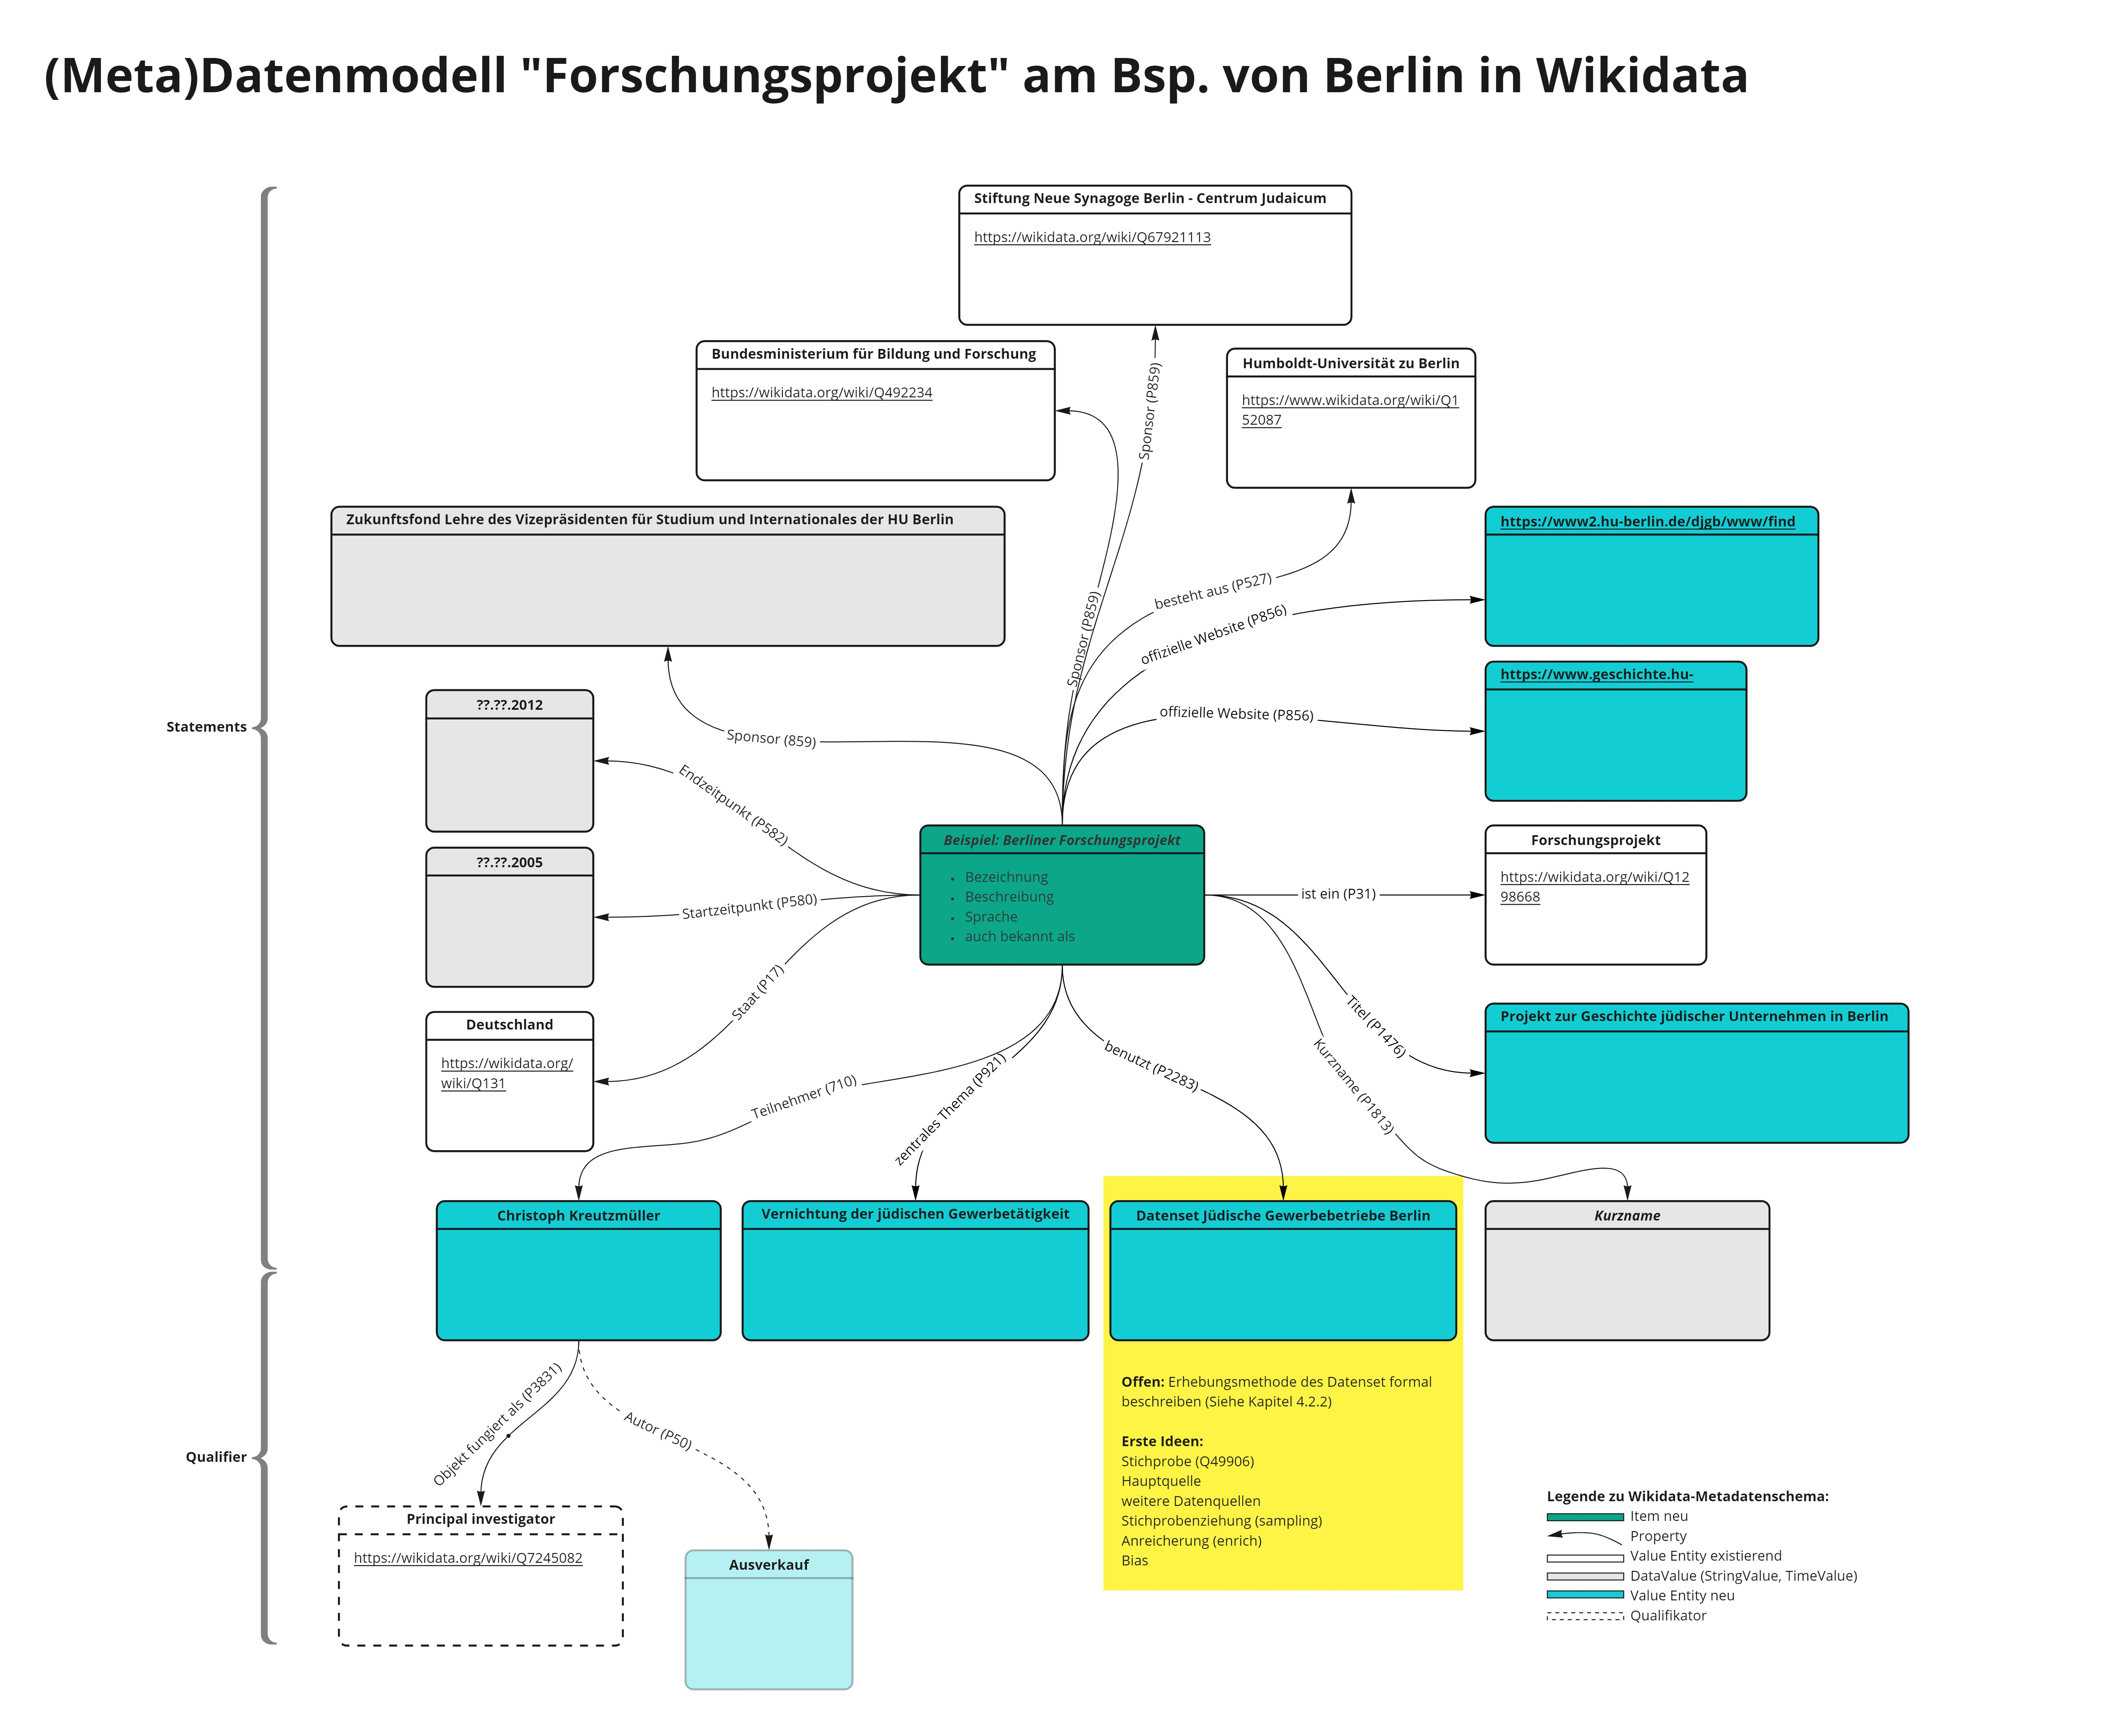
\includegraphics[width=\ScaleIfNeeded]{wikidata-item_research-project}}
    \caption{Modellierung der Forschungsprojekte in Wikidata.}
    \label{fig:x cubed graph} \footnotetext{Größere Darstellungen der Modellabbildungen sind alle separat nochmals im Anhang beigefügt.}
\end{figure}

Folglich wäre die eigene Modellierung von ,,Forschungsprojekt'' für die lokalen Forschungsprojekte im Forschungsfeld redundant, da diese von dem bestehenden Wikidata-Projekt abgeleitet werden kann (Abbildung 4.1).\footnote{Als Orientierung diente das Forschungsprojekt ,,Amyloid fibril cytotoxicity: new insights from novel approaches'', URL: \url{https://www.wikidata.org/w/index.php?title=Q52268104&oldid=1528020632}.} Aus dem Modell in Abbildung 4.1 geht darüber hinaus hervor, dass viele Entitäten in Wikidata bereits existieren und nicht neu angelegt werden müssen.\footnote{Entitäten mit weißem Hintergrund.} Auch die Verknüpfung von externen Information ist möglich. Die Deutsche Forschungsgemeinschaft (DFG) hat mit dem Informationssystem ,,GEPRIS – Geförderte Projekte der DFG'' (GEPRIS)\footnote{URL: \url{https://gepris.dfg.de/gepris/OCTOPUS?task=showAbout} (letzter Zugriff am 21.05.2022).} in Auszügen ihre Daten zu allen gegenwärtigen und vergangenen geförderten Projekten veröffentlicht. Dort ist auch das Forschungsprojekt ,,Geschichte mittlerer und kleiner jüdischer Unternehmen in Frankfurt am Main und Breslau 1929/39 bis 1945'' archiviert.\footnote{URL: \url{https://gepris.dfg.de/gepris/projekt/48308995?context=projekt&task=showDetail&id=48308995&} (letzter Zugriff am 23.05.2022). Hieraus ging u.a. die Lokalstudie zu Frankfurt am Main hervor sowie die im Interview erwähnte Access-Datenbank mit ca. 3.000 Gewerbebetrieben in Frankfurt a.M., Siehe Nietzel 2012 und Interview B2\_Transkript, Pos. 27.} Mit der vorhandenen Wikidata-Property ,,GEPRIS ID (Projekt) (P4870)'', kann demnach das DFG-Projekt mit dessen eindeutiger nummerischer DFG-Kennung ,,48308995'' in Wikidata verknüpft werden.\footnote{Auch die Freie Universität Berlin führt ein zentrales Projektverzeichnis mit detaillierten Informationen zu den einzelnen Projekten, siehe URL: \url{https://research.zuv.fu-berlin.de/projects} (letzter Zugriff am 24.05.2022).}  

Insgesamt ist diese Vorgehensweise zeitsparender, da sich wegen des außerordentlichen Wikidata-Umfangs eine Menge Nachnutzungsmöglichkeiten bieten. Diese Form der Nachnutzung trägt außerdem zur Qualitätsicherung in Wikidata bei. Zudem können erstmals Projekt-Daten aus unterschiedlichen Quellen in Wikidata zusammengeführt und auf diese Weise Informationen vernetzt werden. Sollten für das Forschungsfeld weitere Informationen notwendig werden, können diese dynamisch ergänzt werden, was wiederum der Vorteil des Linked Data-Konzept gegenüber einer herkömmlichen relationen Modellierung in einer SQL-Datenbank ist. Dort ist diese Flexibilität nicht gegeben. Dadurch, dass die Forschungsprojekte als eigene Wikidata-Items nun einen eindeutigen Wikidata-Identifikator besitzen, können sie den zugehörigen Forschungsdaten zugeordnet werden, womit der projektbezogene Entstehungsrahmen erstmals transparent wird.

\subsection{Erhebungsmethode}

Da die methodischen Vorgehensweisen der verschiedenen Wissenschaftsdisziplinen voneinander abweichen, existieren zu deren formalen Beschreibung keine disziplinübergreifenden Metadatenstandards.\footnote{Vgl. forschungsdaten.info, URL: \url{https://www.forschungsdaten.info/themen/beschreiben-und-dokumentieren/metadaten-und-metadatenstandards/} (letzter Zugriff am 15.05.2022).} Das heißt, diese als Prozessmetadaten bezeichneten Daten sind fachspezifisch. Im naturwissenschaftlichen Bereich und in der Archäologie gibt es mit der \textit{Research Resource Identification Initiative} (RRI)\footnote{} und mit \textit{IANUS}\footnote{URL: \url{https://ianus-fdz.de/}. Der Support war nach Auslaufen der DFG-Projektförderung 2017 allerdings eingeschränkt. So konnten neue Datensammlungen bis 2022 nicht aufgenommen werden, siehe URL: \url{http://datenportal.ianus-fdz.de/pages/information.jsp\#dateneigentuemer} (alle letzter Zugriff 15.05.2022).} bereits zentrale Ansätze, wie Methodiken schematisch und anhand von Thesauri oder festen Vokabularen formal beschrieben werden können.\footnote{Siehe zum Beispiel die Thesauri des Deutschen Archäologischen Instituts, URL: \url{http://thesauri.dainst.org/de.html} mit der Kollektion zu den Methoden, URL: \url{http://thesauri.dainst.org/de/collections/\_203bcc05.html} (alle letzter Zugriff am 15.05.2022).} Allerdings sind sie nicht übertragbar auf den geschichtswissenschaftlichen Bereich. Offenes Forschungsdatenmanagement ist hier mit zwei Herausforderungen konfrontiert. Erstens gibt es einen fachspezifischen Standard für die Geschichtswissenschaften nicht. Zweitens ist fraglich, wie sich die Erhebungsmethoden im Forschungsfeld formalisieren lassen. Als Einstiegspunkt soll hier der Versuch einer groben Schematisierung der methodischen Vorgehensweise anhand der Lokalstudien, welche systematisch Daten zu jüdischen Gewerbebetrieben erhoben haben, vorgenommen werden.\footnote{Das sind zuvorderst die Studien zu Hamburg, Berlin, Frankfurt am Main, München, Mannheim und Krefeld.} Zunächst ist festzuhalten, dass die Datenanalyse und -auswertung aller Studien auf Stichprobenziehung beruhte.\footnote{Interessant ist, dass alle Studien mit dem Anspruch gestartet sind, die Gesamtzahl jüdischer Gewerbetriebe zu erfassen. Dieser war allerdings von keiner Studie einlösbar, da erstens das Ausmaß der Zerstörung unterschätzt wurde und zweitens die Projektlaufzeit für eine Totalerhebung zu kurz war, vgl. Interview B3\_Transkript, Pos. 11 und B2\_Transkript, Pos. 23.} Festzustellen ist weiterhin, dass die Überlieferung überall als disparat und lückenhaft bezeichnet wurde, da viele Bestände teilweise oder überwiegend von den Nationalsozialisten vernichtet wurden, um Spuren zu verwischen, oder in den letzten Kriegstagen unwiederbringlich zerstört wurden. Oft sind nur Überreste und Splitter erhalten. Abbildung 4.2 zeigt einen idealtypischen Ablauf der Datenerhebung im Forschungsfeld. Demnach wurde eine Hauptquelle (Datenquelle 1) ausgewählt, aus der ein Sample gezogen wurde.\footnote{In München wurde jeder zweite Buchstabe aus der Gewerbekartei mit jüdischen Gewerbebetrieben erfasst, also ca. die Hälfte der Gewerbebetriebe, vgl. Rappl 2000, S. 179 Fußnote 217. In Frankfurt diente ebenfalls der Bestand aus dem Gewerbeamt als Hauptquelle (vgl. Interview B2\_Transkript, Pos. 31 und 45.), während in Mannheim das Verzeichnis jüdischer Gewerbetreibender sowie alle Arisierungsakten ab 1938 erhalten ist, vgl. Interview B3\_Transkript, Pos. 43 und 47 erhalten sind. In Hamburg basierte die Stichprobenziehung im Wesentlichen auf den Wiedergutmachungsakten, vgl. Bajohr 1998, S. 21ff. und Interview B1\_Transkript, Pos. 33.} In den meisten Fällen konnten daraus die wesentlichen Grunddaten (Name, Inhaber, Branche und Adresse) der Gewerbebetriebe erfasst. Ausgangspunkt bildeten im Idealfall publizierte und unpublizierte Verzeichnisse, Listen oder Karteisammlungen in denen Gewerbebetriebe dezidiert und systematisch mit dem Ziel der Verfolgung als jüdisch markiert und gelistet wurden.\footnote{In München übernahm diese Aufgabe das städtische Gewerbeamt, vgl. Rappl 2000, S. 145f. In Frankfurt am Main war der zentrale Akteur die Industrie- und Handelskammer.} Im nächsten Schritt wurden diese Daten mit weiteren Quellen abgeglichen, die den Vorgang der Verfolgung der einzelnen Gewerbebetriebe verwaltungsseitig dokumentierten. Zu dieser zweiten Datenquelle gehören verschiedene zeitgenössische Aktenbestände.\footnote{Zum Beispiel die Handelsregisterakten, die sogenannten Entjudungsakten oder die Akten der Devisenstellen, aber auch die Wiedergutmachungsakten nach 1945.} Aus diesem Rahmen fällt das Berliner Forschungsprojekt, wo man einen gänzlich anderen Ansatz verfolgt hat. Mangels überlieferter Quellen, wurde ein Sample anhand der Zentralhandelsregisterbeilage (ZHRB) erstellt und aus dieser die Aktivitäten aller handelsregisterlich geführten Unternehmen zwischen 1932 und 1942 erfasst. Man nahm hier folglich eine Gesamtaufnahme des Handelsregisters vor, welches im zweiten Schritt nacheinander mit weiteren Quellen abgeglichen und bei einer eindeutigen Indizienlage Gewerbebetriebe als jüdisch identifiziert wurden.\footnote{Der Autor beschreibt dieses unkonventionelle Vorgehen im Forschungsfeld sehr detailliert in der Einleitung seiner Studie, vgl. Kreutzmüller 2012, S. 29-38.} Auch wenn mit ca. 8.000 identifizierten jüdischen Gewerbebetrieben nur etwa 16 Prozenzt der insgesamt in Berlin ansässigen jüdischen Gewerbebtriebe erhoben werden konnte, stellt das Sample in Bezug auf das Handelsregister als Grundgesamtheit fast eine Vollerhebung dar.\footnote{Von der Forschung wird geschätzt, dass in Berlin rund die Hälfte der jüdischen Gewerbebetriebe im Deutschen Reich ansässig war, also rund 50.000. Kreutzmüller geht von ca. 10.000 im Handelsregister eingetragenen jüdischen Gewerbebetrieben aus, vgl. Kreutzmüller 2012, S. 102f.}

\begin{figure}[h]
    \centering
    \frame{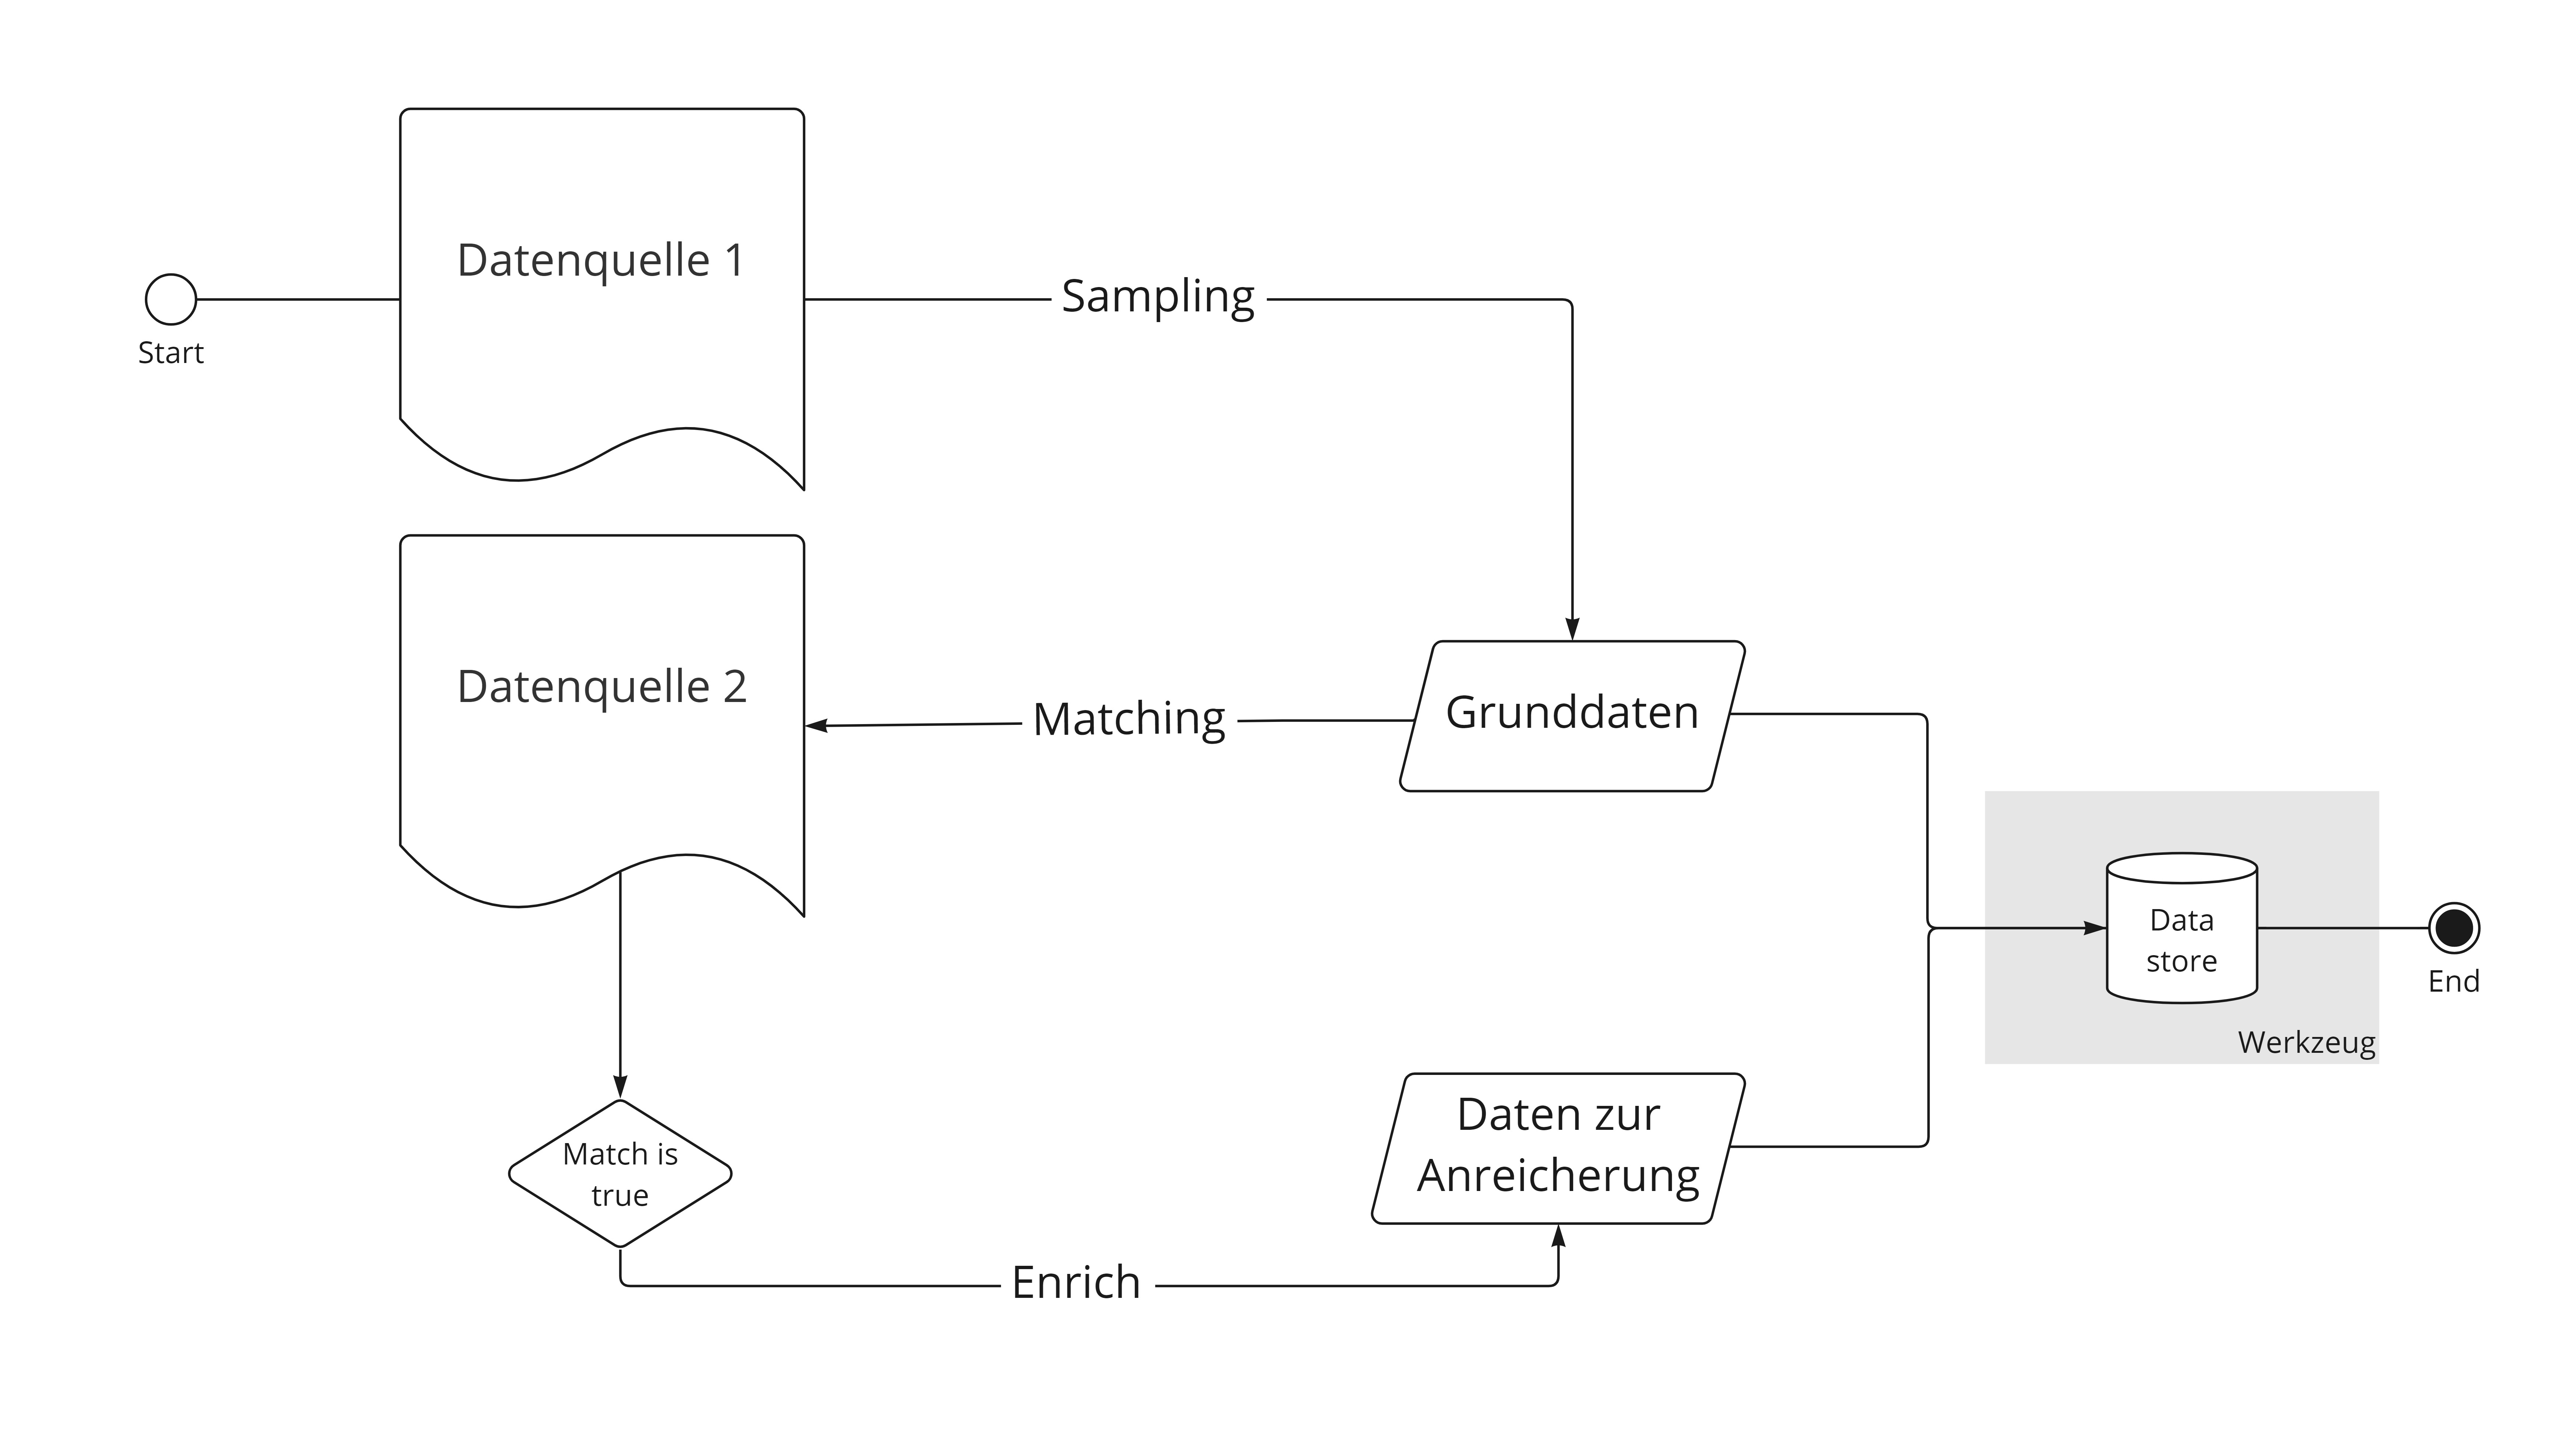
\includegraphics[width=\ScaleIfNeeded]{flowchart_data-collection.jpg}}
    \caption{Idealtypische Stichprobenziehung von Daten zu jüdischen Gewerbebetrieben.}
    \label{fig:x cubed graph}
\end{figure}

Nachteil der vereinfachten, groben Schematisierung ist, dass diese Detailinformationen nicht enthalten sind. Darüber hinaus fehlen die mit der Quellenlage einhergehenden Stichproben-Verzerrungen (Bias) der Studien, welche bisher überhaupt nicht kommuniziert werden:

\begin{itemize}
    \item Viele Hauptquellen setzen zeitlich erst mit den reichsweiten Gesetzen ab 1938 ein. Die frühe Phase der Vernichtung der jüdischen Gewerbetätigkeit bleibt somit unterrepräsentiert, weil schlichtweg Daten dazu fehlen.
    \item Bei der Verwendung von überwiegend Wiedergutmachungsakten, insbesondere aus Rückerstattungsverfahren wie in Hamburg, liegt der Schwerpunkt automatisch auf den größeren Unternehmensverkäufen und den ehemaligen Eigentümern, die den Nationalsozialismus meist durch Emigration überlebt haben. Liquidationen bleiben in diesem Ansatz unterrepräsentiert sowie der komplette Ostteil Deutschlands, da hier die Wiedergutmachung erst in den 90er Jahren mit dem Ende der DDR teilweise einsetzte.
    \item In Berlin wiederum liegt der Fokus mit der ZHRB auf den handelsregisterlich eingetragenen Firmen und damit auf mittelständischen Gewerbebetrieben, wodurch vor allem Kleinstunternehmen unterrepräsentiert bleiben. Außerdem liegt der Schwerpunkt auf Liquidationen, da das Handelsregister Besitzübernahmen nicht abbildet.
\end{itemize}

Es wird deutlich, dass geschichtswissenschaftliche Datenerhebungsmethoden aufgrund der historischen Quellengrundlage nicht analog zu den naturwissenschaftlichen Methoden standardisiert werden können. Es ist die Lückenhaftigkeit und es sind die Fehlstellen in der historischen Forschung, die eine adäquate Abbildung auf ein festes Schema zu einer spezifischen Herausforderung im Fach machen. Daher stellt sich insbesondere auch die Frage, welche Notwendigkeit Standardisierung hier besitzt. Es wäre genauer zu untersuchen, was der Mehrwert davon für die historische Forschung wäre oder ob zum Zwecke der methodischen Transparenz und Nachvollziehbarkeit eine rein textuelle Beschreibung oder Dokumentation zum Beispiel in Form einer Readme-Datei ausreicht. Tatsache ist, dass die Ausführungen zur Erhebung in die einzelnen Lokalstudien bisher unterschiedlich ausfallen und entscheidenden Informationen zum Verständnis der Forschungsdaten ganz fehlen. Auch im Sinne der Nachnutzbarkeit von historischen Forschungsdaten ist also die offene Frage, welche Informationen zur Methodik überhaupt benötigt werden.

\section{Aufbereitung}

\begin{quote}
    [...] Die Datenbank ist ja auch deshalb - ich sag mal erratisch, weil ich sie nur immer mal wieder anpassen konnte. Also alle drei vier Monate kam dann jemand und hat mir geholfen. Und dann hatte ich aber schon drei, vier Monate weitergearbeitet, oder wir. Und dann irgendwie krumm eingeben oder irgend so ein Feld mal benutzt.\footnote{Interview B1\_Transkript, Pos. 3.}
\end{quote}

Um eine valide Datengrundlage für die Analyse zu erhalten, werden die erhobenen Rohdaten vorab aufbereitet. Damit erfolgt erstmalig eine Verarbeitung der Daten, denn der Operationalisierung der Forschungsfragen entsprechend werden die Rohdaten ausgewählt, erfasst und bereinigt. In der historischen Forschung liegt die Situation vor, dass die Rohdaten im Quellenmaterial zwar bereits vorliegen, sich aber mitunter über viele Quellen verteilen. Daher muss festgelegt werden, erstens welche Informationen aus den Quellen extrahiert und erfasst werden sowie zweitens, mit welchem Werkzeug diese zusammengeführt werden sollen. Dieser Prozess der Forschungsdaten-Genese ist bisher im Forschungsfeld weitestgehend unsichtbar und findet lediglich in den Studien zu Berlin und Frankfurt am Main nachträglich in den Publikationen Erwähnung.\footnote{Vgl. Kreutzmüller 2012, S. 38f., Nietzel 2012, S. 17.}. In beiden Projekten kamen ,,Datenbanken'' zum Einsatz, die anhand der Interviews als Microsoft Access-Datenbanken der Version 2007 spezifiziert werden konnten.\footnote{Vgl. Interview B2\_Transkript, Pos. 27.} Da es sich hierbei um eine Anwendung handelt, deren Datenorganisation auf relationalen Tabellen beruht, braucht es als Basis vorab ein Datenmodell, visualisiert zum Beispiel anhand eines Entity-Relationship-Diagramms (ERD) mit einer Beschreibung der darin verwendeten Elemente. Dieses ist für beide Studien allerdings nicht verfügbar. Damit ist eine Beurteilung der Daten hinsichtlich ihrer Verarbeitung für alle Lokalstudien bisher nicht möglich. Ziel von offenem Forschungsdatenmanagent ist es daher, die Phase der Aufarbeitung transparent zu machen und Zusammenarbeit zwischen den Projekten zu ermöglichen. 

Zu diesem Zweck wurde in Wikidata das Projekt \textit{Wikidata:WikiProject Destruction of the Economic Existence of the Jews Research} erstellt (Abbildung 4.3.).\footnote{URL: \url{https://www.wikidata.org/wiki/Wikidata:WikiProject_Destruction_of_the_Economic_Existence_of_the_Jews_Research}.} Dieses besitzt grob drei Funktionen: Erstens können beliebig viele Seiten mithilfe von standardisierten Templates hierarchisch im Projekt angelegt werden (Pages und Subpages).\footnote{Siehe URL: \url{https://www.mediawiki.org/wiki/Help:Templates} (letzter Zugriff am 24.05.2022).} Diese bieten die Möglichkeit, die in Kapitel 3 methodisch aufgegriffene Taxonomie und damit die unterschiedlichen Zugänge im Forschungsfeld funktional umzusetzen. Auf der Hauptseite (Home) wurden bereits Hintergrundinformatioen zum Projekt sowie zu dessen Zielen hinzugefügt. Dort ist auch erwähnt, dass diese Arbeit nur den Ausgangspunkt bildet und von hier aus sukzessive die angrenzenden Untersuchungsbereiche integriert werden können. Außerdem findet sich hier die nicht unwichtige Information, dass die Taxonomie im Forschungsfeld dem Systematisierungversuch von Nietzel aus dem Jahr 2009 entlehnt ist.\footnote{Siehe Kapitel 3.2.1.}    

\begin{figure}[h]
    \centering
    \frame{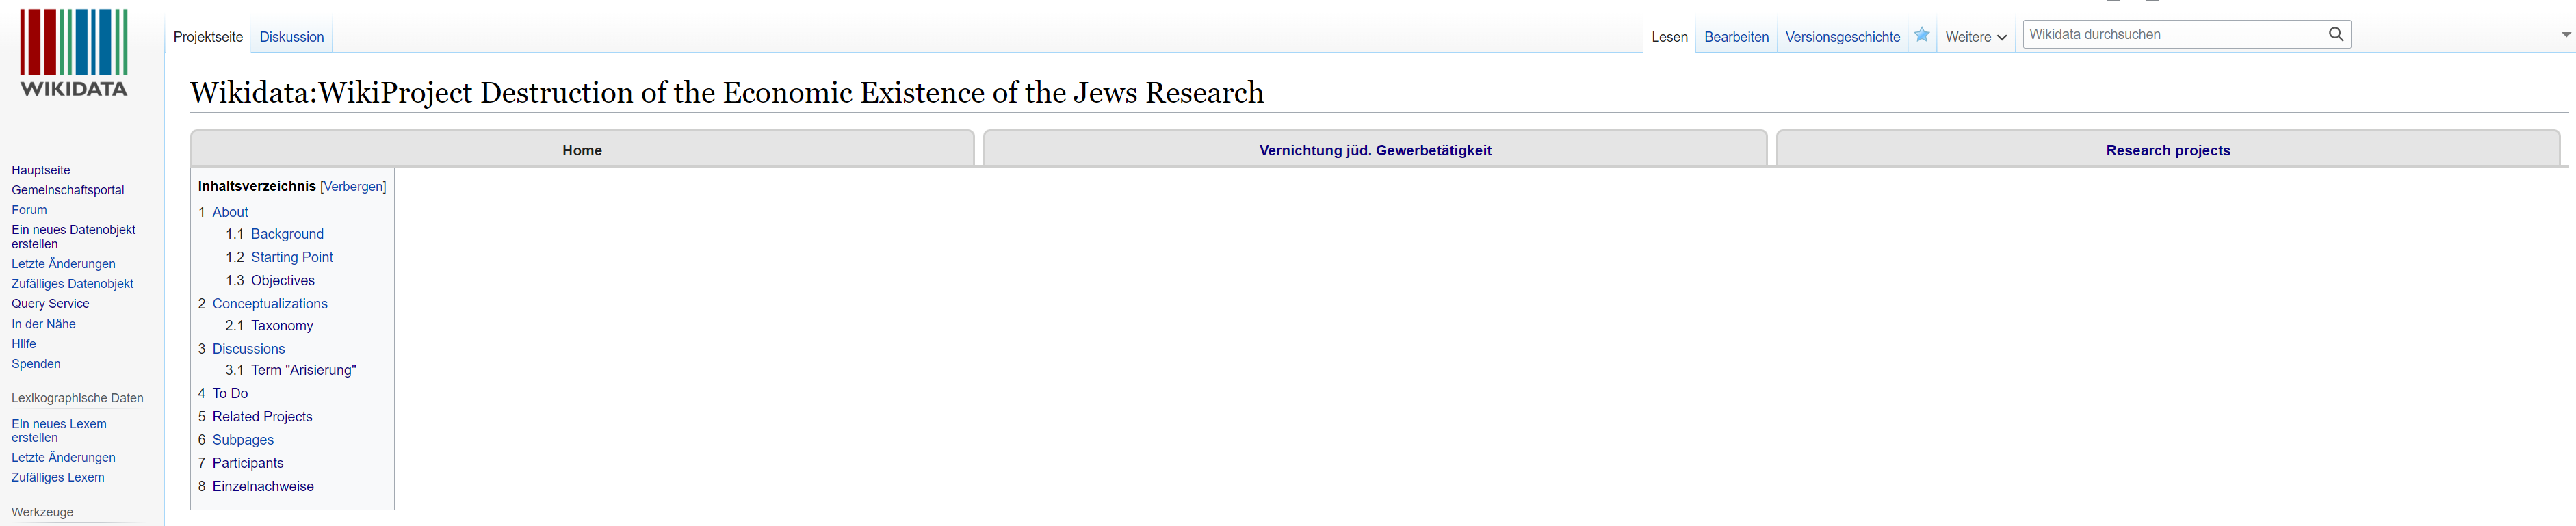
\includegraphics[width=\ScaleIfNeeded]{wikidata-project_tabs}}
    \caption{Wikidata:WikiProject Destruction of the Economic Existence of the Jews Research mit den in Tabs angelegten Subpages.}
    \label{fig:x cubed graph}
\end{figure}

Die bisherige Implementierung versteht sich explizit als Vorschlag, um eine Ausgangsbasis zu haben, von der aus Anpassungen und Weiterentwicklungen möglich werden. Um später in den gemeinsamen Austausch zu treten und Änderungen vorzunehmen, kann hierfür die zweite grundlegende Funktion der Diskussionseiten genutzt werden. Schließlich gibt es mit der Versionierung (,,Versionsgeschichte'') eine Kontrollfunktion, mit der sich alle Bearbeitungen zurückverfolgen und gegebenfalls auf einen früheren Stand zurücksetzen lassen.\footnote{URL: \url{https://www.wikidata.org/w/index.php?title=Wikidata:WikiProject_Destruction_of_the_Economic_Existence_of_the_Jews_Research&action=history} (letzter Zugriff am 24.05.2022).} Ingesamt bietet das Wikidata-Projekt damit die Möglichkeit des kollaborativen Austauschs und der gemeinsamen Strategieentwicklung im Forschungsfeld. Erstmals können Methodiken und Konzepte im Forschungsfeld diskutiert sowie in Bezug auf die in der Arbeit betrachteten Forschungsdaten ein allgemeingültiger Leitfaden zur Erfassung jüdischer Gewerbebetriebe entwickelt werden. Thematisch ist das Wikidata-Projekt in die Kategorien \textit{History WikiProjects} und \textit{Research WikiProjects} eingeordnet.\footnote{Siehe Wikidata:WikiProjekte, URL: \url{https://www.wikidata.org/wiki/Wikidata:WikiProjects/de} (letzter Zugriff am 24.05.2022).} Hier zeigt sich darüber hinaus, dass benachbarte Forschungsfelder zum Nationalsozialismus und zum Holocaust bereits mit eigenen Projekten vertreten sind, womit sich Anknüpfungspunkte über das Forschungsfeld hinaus ergeben.\footnote{Siehe WikiProject WWII, URL: \url{https://www.wikidata.org/wiki/Wikidata:WikiProject\_WWII}; WikiProject NS Perpetrator Research, URL: \url{https://www.wikidata.org/wiki/Wikidata:WikiProject\_NS\_Perpetrator\_Research}; WikiProject Victims of National Socialism, URL: \url{https://www.wikidata.org/wiki/Wikidata:WikiProject\_Victims\_of\_National\_Socialism}; WikiProject NS-Täterforschung, URL: \url{https://www.wikidata.org/wiki/Wikidata:WikiProject\_NS-Täterforschung}; Wikidata:WikiProject Nuremberg Trials, URL: \url{https://www.wikidata.org/wiki/Wikidata:WikiProject\_Nuremberg\_Trials} (alle letzter Zugriff am 24.05.2022).} 

\subsection{Problem \textit{Jüdischer} Gewerbebetrieb}

Da Untersuchungsgegenstand aller Lokalstudien ,,Jüdische Gewerbebetriebe'' oder ,,Jüdische Unternehmen'' sind, wurde folglich Daten zu jüdischen Gewerbebetrieben erfasst. Hieraus ergibt sich eine grundlegende methodische Schwierigkeit: Da die Konfessionszugehörigkeit bezüglich eines Gewerbebetriebs oder Unternehmens schlichtweg unlogisch ist, ist der Begiff alleine ohne Kontext unbrauchbar. Dieses Problem wird von dem meisten Studien reflektiert und betont, dass es sich hierbei um eine antisemitische Zuschreibung und Konstruktion handelte. Diese Kennzeichnung und Diffamierung diente den Nationalsozialisten als Instrument für die weiteren Verfolgungspraktiken. Zur einfacheren Handhabung wurde der Begriff als Quellenbegriff jedoch von allen Studien beibehalten. Hierbei fallen zwei unterschiedliche Verwendungen auf: 

\begin{itemize}
    \item Der Begriff ,,jüdischer Gewerbebetrieb'' wird ausschließlich auf die jüdischen Besitzer*innnen bezogen und angewandt.\footnote{Vgl. Janetzko 2012, S. 18.} Damit wird jedoch das methodische Problem nicht aufgelöst, sondern verlagert sich auf den Begriff ,,jüdische Person'' oder ,,Jude/ Jüdin'', bei dem es sich ebenfalls um eine rassistische Zuschreibung handelte und nichts mit dem Selbstverständnis der Betroffenen zu tun hatte.\footnote{Das wird in der Studie zu Hamburg auch ausführlich reflektiert. Vgl. Bajohr 1997, S. 9.} Darüber hinaus werden in dieser Verwendung weitere Verfolgungskontexte vernachlässigt. So war es in der frühen Phase der Verfolgung durchaus möglich, dass Gewerbebetriebe als jüdisch diffamiert wurden, die zum Beispiel einen hohen Anteil jüdischer Mitarbeiter*innen aufwiesen, deren Besitzer aber selbst nach der nationalsozialistischen Ideologie nichtjüdisch waren.\footnote{An diesem Beispiel zeigt sich überdies die in Wechselbeziehung stehenden Teilprozesse der Verdrängung der Juden aus dem Berufsleben und der Vernichtung der jüdischen Gewerbetätig deutlich.}
    \item Der Begriff ,,jüdischer Gewerbebetrieb'' wird mit ,,als jüdisch betrachtet/ verfolgt'' übersetzt. In dieser Verwendung ist die jüdische Eigentümerschaft eines Gewerbebetriebs zunächst unerheblich, das heißt sie wird nicht vorausgesetzt, sondern es werden alle Gewerbebetriebe erfasst, die im nationalsozialistischen Kontext diffamiert wurden. Damit wird einerseits der Konstruktioncharakter des Begriff hervorgehoben und andererseits dem Umstand Rechnung getragen, dass die rassistischen Zuschreibungen grundsätzlich jeglicher rationalen Begründung entbehrten und aus diesem Grund willkürlich erfolgen konnten.
\end{itemize}

Auch wenn in allen Studien der selbe Untersuchungsgegenstand genannt wird, so zeigt sich erst in der konkreten Verwendung, dass dieser unterschiedlich ausgedehnt werden konnte, weil der Begriff an sich nicht widerspruchsfrei ist. Aus forschungsethischer Perspektive ist zudem problematisch, dass ein rassistisch konnotierter Begriff in der wissenschaftlichen Forschung beibehalten wird. Wichtig wäre, sich im Forschungsfeld auf eine einheitliche Verwendung zu einigen, denn bisher werden Daten zu jüdischen Gewerbebetrieben unterschiedlich erhoben und erfasst. 

Hierzu wird im Rahmen dieser Arbeit keine abschließende Aussage getroffen, da dies in einem Diskurs im Forschungsfeld gemeinsam entschieden werden sollte. Um dafür den Anstoß zu geben, wurde im Wikidata-Projekt der \textit{Wikidata talk} ,,How do we use and model ,Jüdischer Gewerbebetrieb'?'' mit der Disskussionsfunktion angelegt und zwei Vorschläge unterbreitet (Abbildung ): 

\begin{itemize}
    \item ,,Jüdischer Gewerbebetrieb'' wird als eigenes Item angelegt und mit Statements angereichert, die das nationalsozialistische Konstrukt deutlich machen. Da in Wikidata Items von jedem/ jeder ohne Einschränkung angelegt werden können, wäre diese Lösung schnell umsetzbar. Bei der Frage mit welcher Eigenschaft (Property) das Item als Value auf einen Gewerbebetrieb abgebildet werden soll, lohnt abermals ein Blick auf benachbarte Wikidata-Projekte. Im Projekt \textit{Wikidata:WikiProject Victims of National Socialism} wurde 2020 die Verwendung des Begriffs ,,Holocaust-Opfer'' diskutiert.\footnote{Wikidata Talk:Q2763 (2020), Modeling of holocaust victim, URL: \url{https://www.wikidata.org/w/index.php?title=Talk:Q2763&oldid=1392179230}}. Da in der Wikidata Konvention ist, Personen so neutral wie möglich zu beschreiben und Zuschreibungen von außen mit entsprechenden Aussagen kenntlich zu machen, hat man sich im Wikidata-Projekt darauf geeinigt, den Begriff nunmehr zusammen mit ,,Subjekt fungiert als (P2868) Opfer des Holocaust (Q5883980)'' zu verwenden und nicht mehr als ,,ist ein(e) (P31) Holocaust-Opfer (Q5883980)''.\footnote{Siehe zum Beispiel Wikidata-Item Anne Frank (Q4583), URL: \url{https://www.wikidata.org/w/index.php?title=Q4583&oldid=1645273699}.} Diese Verwendung kann für Gewerbebetriebe übernommen werden. Zwar geht es hier ausdrücklich nicht um Personen. Da aber die Verwendung ,,ist ein(e) (P31) Jüdischer Gewerbebetrieb (Q???)'' - wie gezeigt wurde - unlogisch wäre, bietet sich ,,Subjekt fungiert als (P2868) Jüdischer Gewerbebetrieb (Q???)'' an.
    \item Statt als Item kann ,,Jüdischer Gewerbebetrieb'' auch als Property ,,als jüdisch betrachtet/ verfolgt (P???)'' oder ähnlich modelliert werden.\footnote{Dieser Ansatz wurde vom Berliner Forschungsprojekt umgesetzt.} Da diese Eigenschaft bisher noch nicht existiert, wäre diese Umsetzung etwas langwieriger, da Eigenschaften in der Wikidata nicht von jedem/jeder erstellt werden, sondern zunächst vorgeschlagen werden müssen.\footnote{Wikidata:Eigenschaften vorschlagen (2022), URL (stable): \url{https://www.wikidata.org/w/index.php?title=Wikidata:Property_proposal/de&oldid=1624532274}.} Nach einer öffentlichen Debatte entscheidet eine berechtigte Administratoren-Gruppe der Wikidata, ob die Property neu aufgenommen wird oder ob Alternativ-Eigenschaften zur Verfügung stehen. Mit diesem Verfahren sollen Redundanzen und Widersprüchlichkeiten verhindert werden. Es dient zur Qualitätskontrolle der Wikidata. Daher ist es möglich, dass für das Forschungsfeld notwendige Eigenschaften für die Wikidata insgesamt nicht die Relevanz besitzen und aus diesem Grund abgelehnt werden können. Wie liberal oder konservativ die Wikidata-Politik hier ist, müsste erprobt werden.      
\end{itemize} 

\begin{figure}[h]
    \centering
    \frame{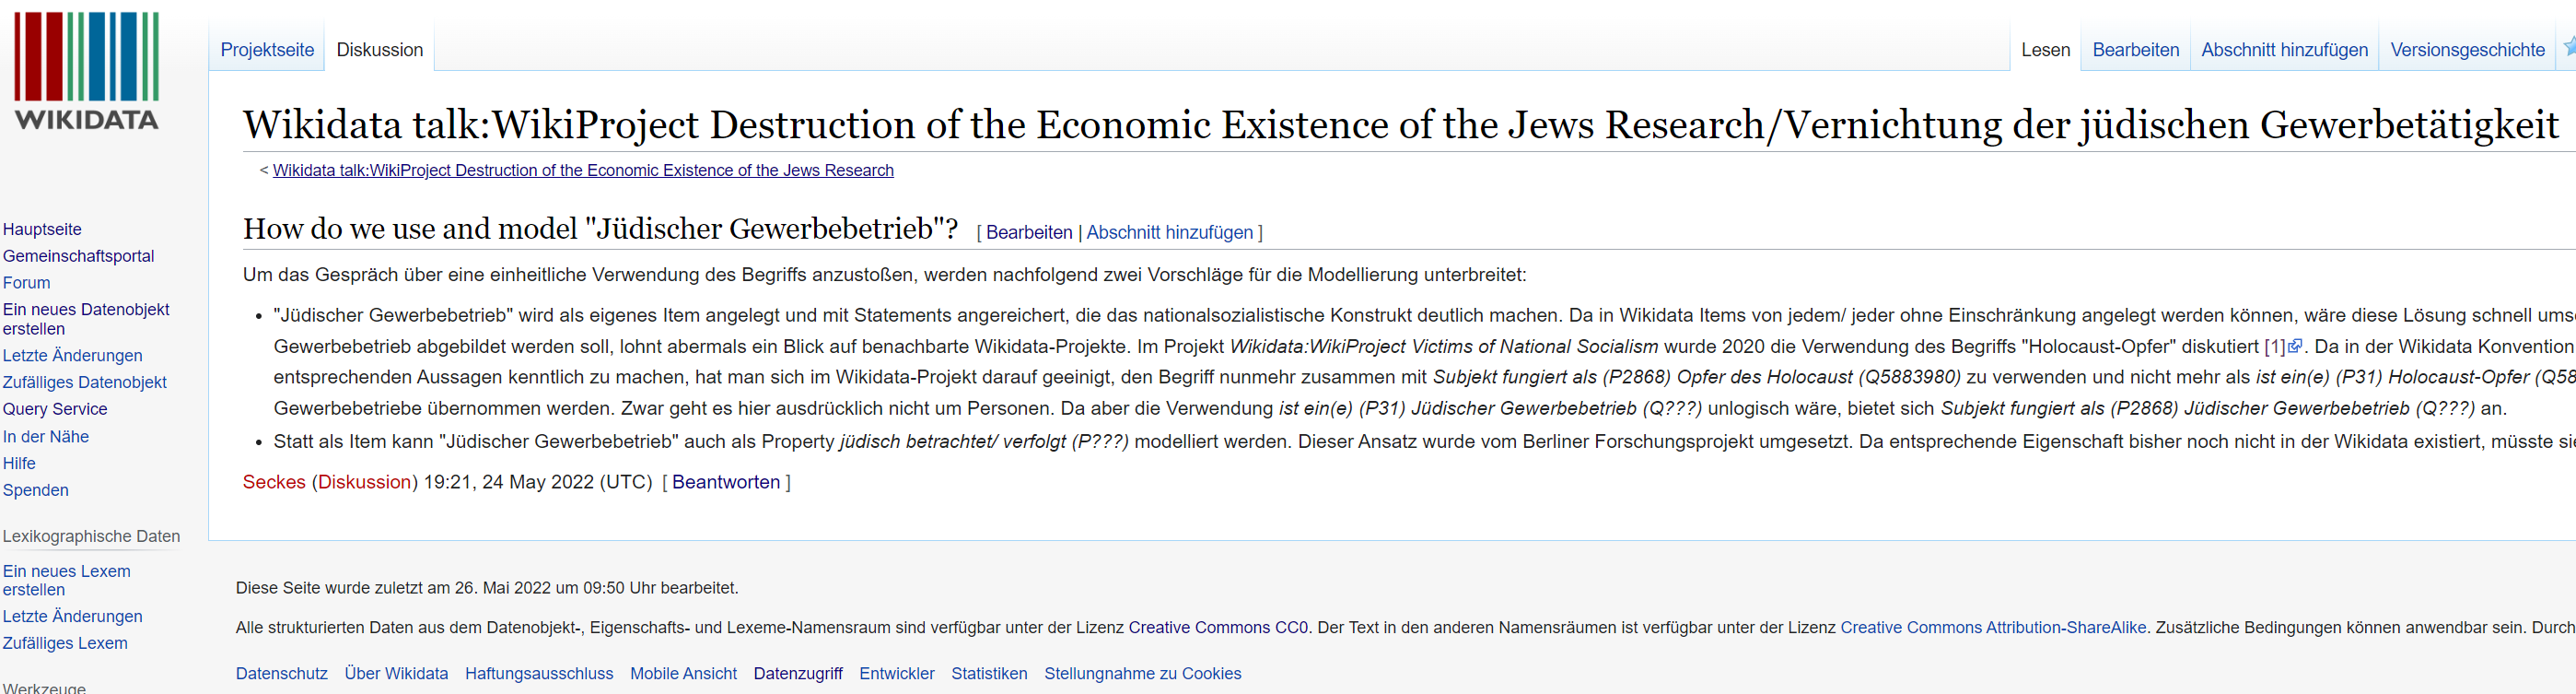
\includegraphics[width=\ScaleIfNeeded]{wikidata-discussion-jued-gewerbebetrieb}}
    \caption{Diskussionsseite zur Frage, wie "Jüdischer Gewerbebetrieb" verwendet und modelliert werden soll.}
    \label{fig:x cubed graph}
\end{figure}

Die funktionale Umsetzung in Wikidata zwingt, ,,Jüdischer Gewerbebetrieb'' als Konzept zu modellieren. Daher wird in beiden Vorschlägen der Ansatz verfolgt, den Konstruktions- und Zuschreibungscharakter des Begriffs sichtbar zu machen und die Verwendung von der den Betrieb inhabenden Person zu entkoppeln, was in Wikidata gut umsetzbar ist. 

\subsection{Zusammenführung der Quellen}

\paragraph{Datenmodell} Beim Zusammenführen der Quellen wurden die ausgewählten verteilten Informationen als strukturierte Daten zentral in Excel oder Access gespeichert. Auch wenn es in den Interviews von keinem Befragten bewusst formuliert wurde, so haben alle zur ,,Handhabbarmachung der Informationen''\footnote{Kreutzmüller 2012, S. 38.} eine \textit{Modellierung} von den zu erfassenden Daten vorgenommen. Bei diesem Vorgang wird ein eindeutig definierter realer Ausschnitt auf ein Modell abgebildet und die enthaltenen Konzepte operationalisiert. Einleitendes Zitat lässt die Vermutung zu, dass ein Datenmodell vorab nicht fixiert wurde, sondern dieses parallel zur Datenerfassung entstand und erweitert wurde.\footnote{Siehe auch Interview B2\_Transkript, Pos. 31 und Interview B1\_Transkript, Pos. 75.} Daraus ergeben sich zwei Anforderungen an offenes Forschungsdatenmanagement: Kollaborative Zusammenarbeit zwischen den Projekten kann nur funktionieren, wenn man sich auf eine Terminologie und auf ein Schema einigt. Es müssen folglich erstens die vielen unterschiedlichen Modelle und Begriffe der einzelnen Studien für eine gemeinsame Nutzung kompatibel gemacht werden. Da aufgrund der besonderen Überlieferungsstruktur ein statisches Modell vorab nicht feststeht, muss dieses zweitens dynamisch und skalierbar sein.
\begin{figure}[h]
    \centering
    \frame{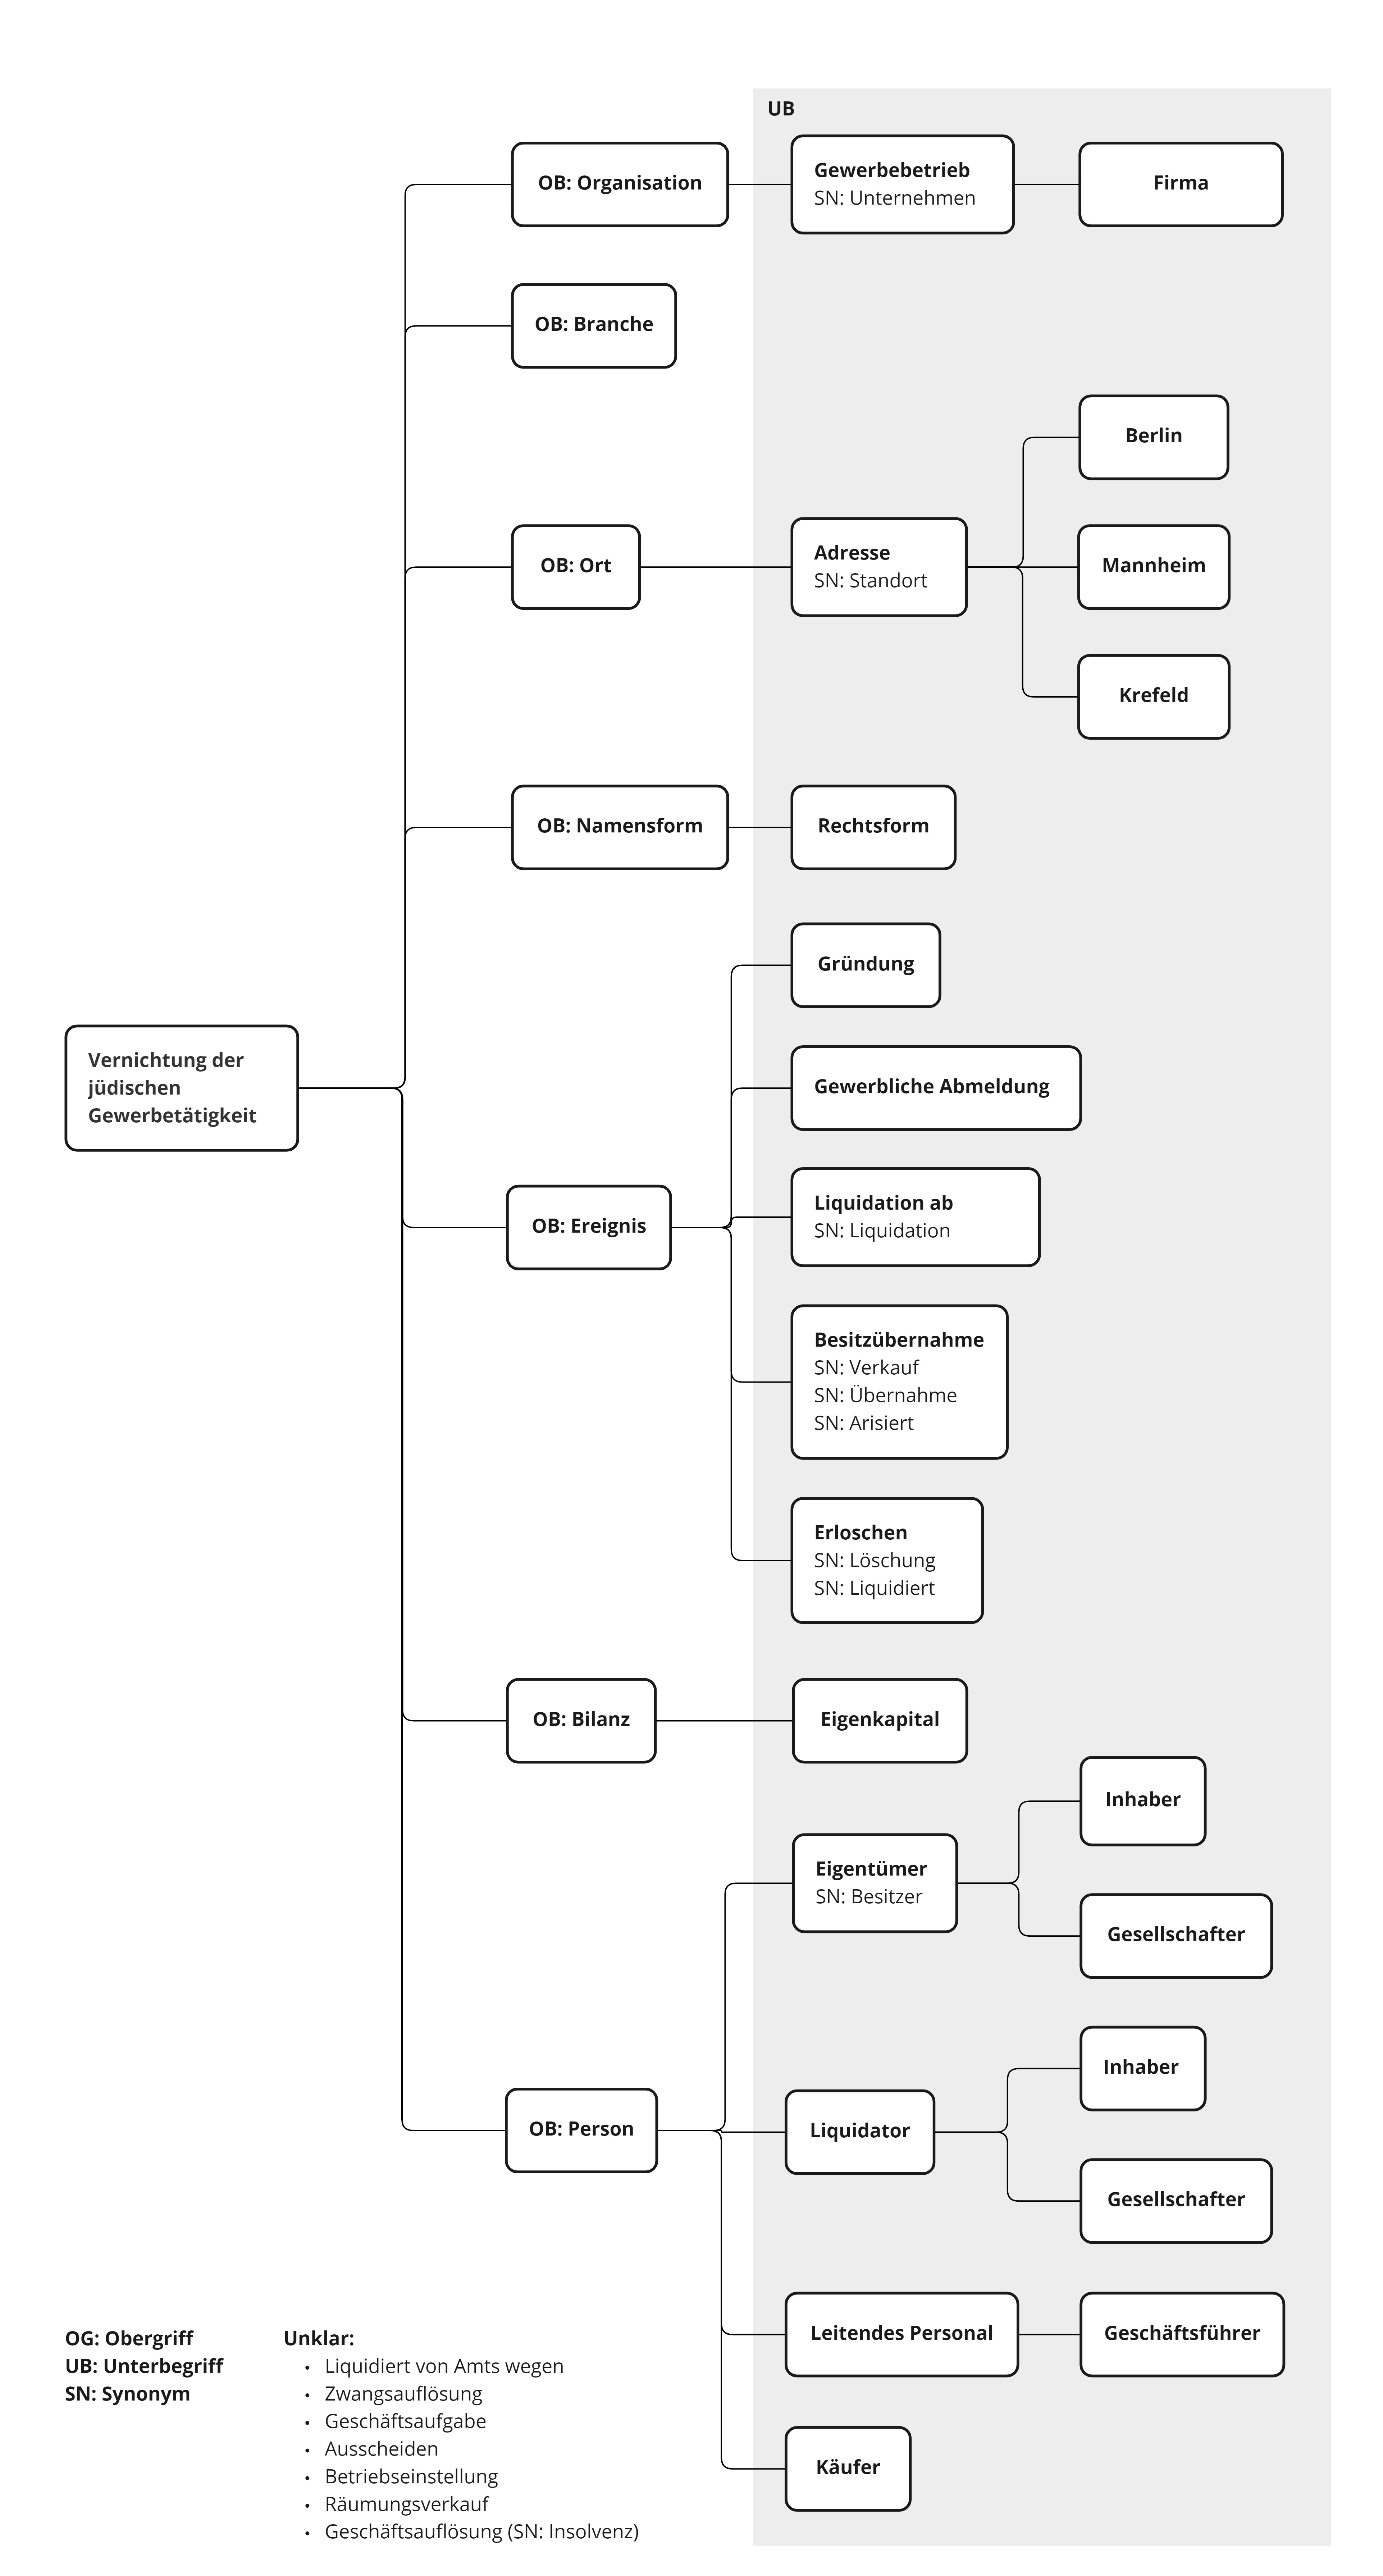
\includegraphics[scale=0.04]{thesaurus}}
    \caption{Sacherschließung des Untersuchungsfelds ,,Vernichtung der jüdischen Gewerbetätigkeit''.}
    \label{fig:x cubed graph}
\end{figure} 
Anhand der für die Arbeit zu Verfügung gestellten Daten aus Berlin, Mannheim und Krefeld sowie mithilfe der Interviews wurde zunächst versucht, eine begriffliche Kontrolle im Untersuchungsfeld zur Vernichtung der jüdischen Gewerbetätigkeit im NS zu erhalten. Hierbei wurde sich der Methodik der Dokumentbeschreibungssprachen aus den Bibliotheks-, Dokumentations- und Informationswissenschaften bedient, mit der Fachgebiete mittels Thesauri oder Klassifikationen hierarchisch geordnet und inhaltlich erschlossen werden (Sacherschließung).\footnote{Siehe Gernot Wersig: Thesaurus-Leitfaden. Eine Einführung in das Thesaurus-Prinzip in Theorie und Praxis, Berlin, Boston 2016, doi:10.1515/9783111412719.} In diesem Sinne wird das Untersuchungsfeld als eigenes Begriffssystem verstanden, mittels dessen es sich inhaltlich beschreiben lässt. Auf diese Weise konnte nicht nur eine Übersicht über die wesentlichen historischen Informationen im Untersuchungsfeld erstellt werden, sondern es zeigte sich mit dieser Methode auch, dass es zum einen Mehrdeutigkeiten bei der Bezeichnung von Sachverhalten gibt (Synonymproblem) und zum anderen Unklarheiten bestehen, wie Begriffe angewandt werden sollen (Abbildung 4.5, grau hinterlegt).\footnote{Ebd., S. 47-51.} Für das Synonymproblem wurden Äquivalenzklassen vorgeschlagen (in den einzelnen Kästchen fett hervorgehoben). Die unklaren Begriffe müssen in dieser Arbeit offen bleiben, da abschließend deren globale Relevanz für das Forschungsfeld nicht bestimmt (z.B. Insolvenz)\footnote{Die Geschäftsauflösung bzw. Insolvenz wurde nur in der Krefelder Studie untersucht.} oder ihre Ambiguität (z.B. Geschäftsaufgabe) nicht aufgelöst werden konnte. 



Das feine Begriffssystem (Abbildung 4.5, grau hinterlegt) wurde auf der ersten Ebene grob abstrahiert. Die generischen Begriffe ergeben damit eine Top-Level-Ontologie für das Forschungsfeld.\footnote{Siehe zu Top-Level-Ontologie Rehbein, Ontologien, 2017, S. 162-174.} Diese kann unabhängig von den Lokalstudie auf alle Forschungsdaten im Forschungsfeld und darüber hinaus angewandt werden. Das bedeutet, das Datenmodell ist offen im Sinne von interoperabel, kann also in der Perspektive auch an benachbarte Forschungsfelder anschließen.



    

\begin{figure}[h]
    \centering
    \frame{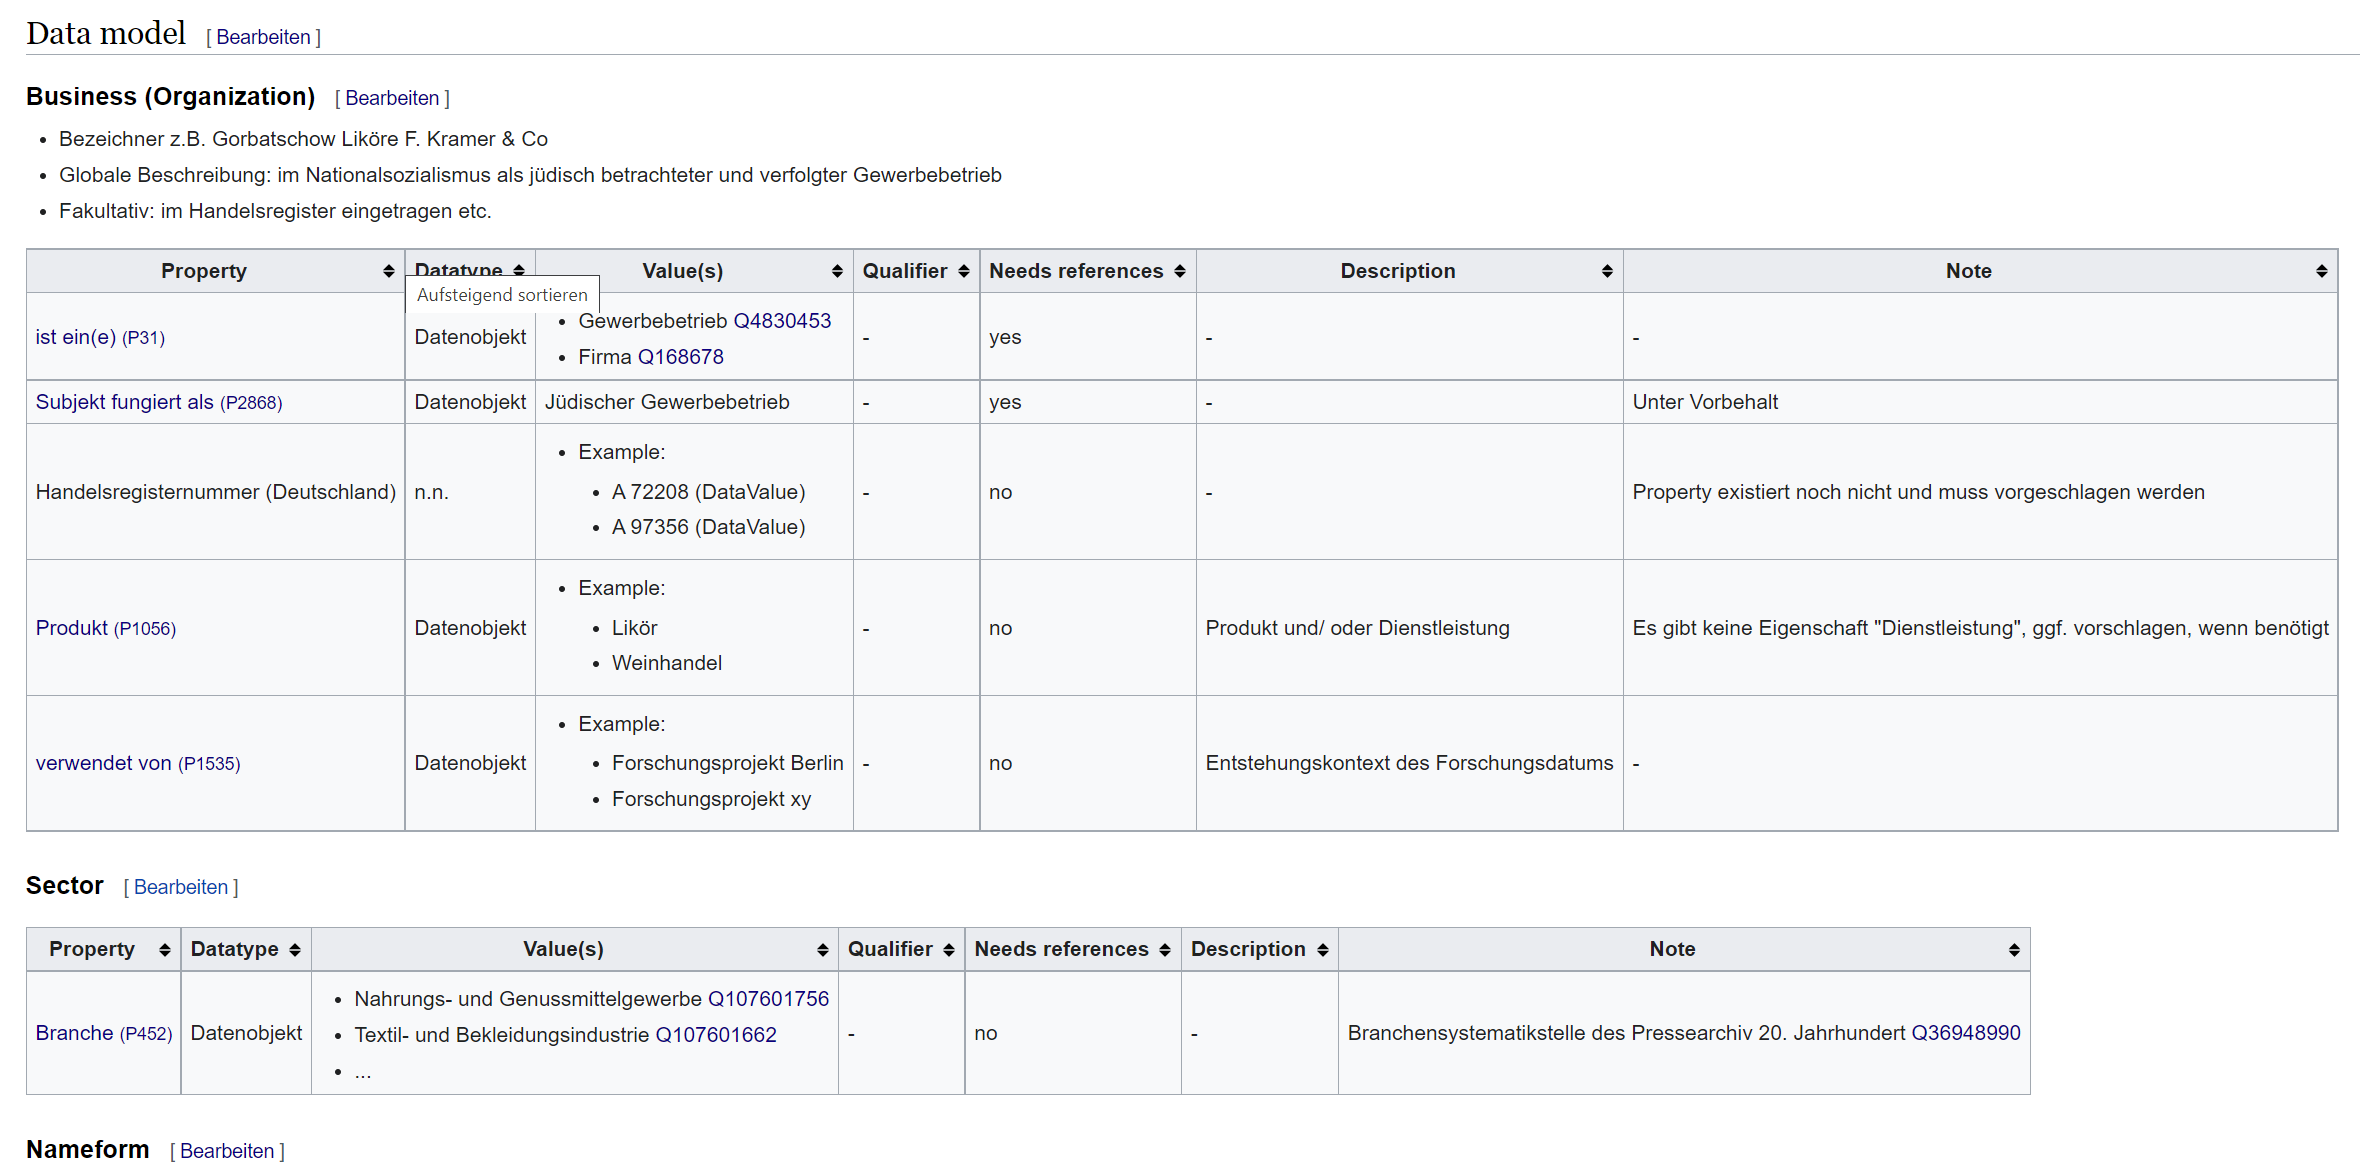
\includegraphics[width=\ScaleIfNeeded]{wikidata-data-model}}
    \caption{Wikidata-Datenmodell für die Forschungsdaten zu jüdischen Gewerbebetrieben.}
    \label{fig:x cubed graph}
\end{figure}




Um die unterschiedlichen Daten aus den einzelnen Lokalstudien kompatibel zu machen, wurde eine  verwendet.  Dise 

In Berlin und Frankfurt a.M. war vordergründig das Ziel, den Prozess der Vernichtung empirisch zu untersuchen, was anhand der Analyseinheiten ,,Gründung'', ,,Besitzübernahme'', ,,Gewerbliche Abmeldung'', ,,Liquidation'' und ,,Erloschen'' erfolgte. Auch hinsichtlich der Gegenstrategien näherte man sich einer quantitativen Auswertung über Namens- und Rechtsformveränderungen. Folglich wurden alle ermittelbaren Namens- Rechtsformen, die ein jüdischer Gewerbebetrieb besaß, erfasst. Um Gewerbestruktur und Verteilungen im Stadtraum zu untersuchen, wurde Branchenzugehörigkeit und Adressen aufgenommen. In der frühen Zeit des Forschungsfelds spielten außerdem die nichtjüdischen Erwerber*innen eine größere Rolle und man versuchte, deren Verhalten mit den Einheiten ,,Stille Teilhaber'', ,,Gutwillige '' und ,,Böswill '' quantifizierbar zu machen.\footnote{Bajohr und Janetzko}



zu erhalten, müssen die verschiedenen Quellen Wie einleitend zu diesem Kapitel bereits beschriebendie Daten aus den verschiedenen Projekten kompatibel machen und Datenmodell so generisch und damit offenen für anderre Forschungsfelder halten
Formale Beschreibung jüdischer Gewerbebetriebe, Relationen, Datensätze zu diesen erstellen --> gibt vor, welche Daten erfasst werden zur inhaltlichen Erschließung


, Modellierunghier konkret zum Datenmodell, jeder sein eigenes Datenmodell, stand mehr oder weniger von Anfang an fest
Bei der Erfassung im Klaren sein, welche Daten ich für Forschungsfrage benötige und welche kassiert werden können
Grunddaten --> Name, Inhaber, Branche, Adresse
weitere ortsbezogene Daten --> Geodaten, mehrere Adressen ermöglichen, wenn es Filialien gab oder bei Umzügen
Eventdaten --> Veränderungen (Prozess der Vernichtung), Namens-Rechtsformveränderungen, Besitzerwechsel, Liquidationen

Herausforderung: Bisher keine festes Vokabular zur Beschreibung, jedes Projekt für sich 

Datenmodell entwickeln, dass für alle Projekte funktioniert, also 
Kompabilität --> Top-Level-Ontologie (stellt Austauschbarkeit sicher)
Inhaltserschließende Metadaten
EntitySchema items, properties, qualifiers und references

während dieser Phase Kollaboration und Diskursabbildung






Es braucht dynamische Umgebung
\paragraph{Quellennachweise}
bibliografische DatenQuellennachweis für Einzeldaten
Nachweis, der einen Gewerbebtrieb als jüdisch identifiziert hat, aus den Interviews ist auch hervorgegangen, dass das nicht immer so eindeutig ist und es keine feste Kriterien gibt. Dies ergibt sich aus bereits erläuterten der methodischen Schwierigkeit in der Verwendung des Begriffs, die sich auch mit einem Forschungsdatenmanagement nicht vollständig auflösen lässt, es scheint aber eben an dieser Stelle umso wichtiger, transparent und nachvollziehbar für jeden zu machen, warum ein Unternehmen als jüdisch identifiziert wurde, dann ist man zumindest in der Lage Grenzfälle, anders als gegenwärtig, wo man den Autoren einfach glauben muss, zu diskutieren bzw. gemeinsam Kriterien zu entwickeln, falls das überhaupt möglich ist.
Verlinkung zu Digitalisaten um hier gemeinsame Qualitätskontrolle zu erhalten, die es bisher ja noch gar nicht gibt

Bibliotheken oder Archiven bei der Katalogisierung 



Es gibt für die einheitliche Beschreibung bereits Metadatenstandards mit fachübergreifende Schemata,  Im wissenschaftlichen Kontext ist ein Trend zu ,,DataCite'' erkennbar.\footnote{Siehe forschungsdaten.info (2022): DataCite-Best-Practice-Guide, URL: \url{https://www.forschungsdaten.info/themen/beschreiben-und-dokumentieren/metadaten-und-metadatenstandards/} sowie Julian Schulz, Sonja Kümmet, Stephan Lücke, Martin Spenger, Tobias Weber (2020): Standardisierung eines Standards: Warum und wie ein Best-Practice-Guide für das Metadatenschema DataCite entstand, Version 1 (20.01.2020, 13:49). In: Korpus im Text, Serie A, 42800Absatz 15. URL: \url{http://www.kit.gwi.uni-muenchen.de/?p=42800&v=1\#p:15} (alle letzter Zugriff am 15.05.2022).} Problematisch ist, das beide Standards zum gegenwärtigen Zeitpunkt nicht als sogenannte Identifiers in Wikidata integriert sind. Daher muss eine Zwischenlösung gefunden werden. Da in Wikidata teilweise auf ,,Dublin Core'' referenziert wird, wird dieses Schema als Orientierung für die formale Beschreibung der projektbezogenen Datenherkunft herangezogen und versucht, auf Entitäten in Wikidata abzubilden (Tabelle ). DataCite ermöglicht seit 2021 ein Mapping des DublinCore-Schemas auf eigene Entitäten, wodurch eine Kompabilität beider Standards gewährleistet ist.\footnote{DataCite Metadata Working Group. (2021). DataCite to Dublin Core Mapping 4.4. DataCite e.V., doi:10.14454/qn00-qx85.}


Es werden also Metadaten zum Forschungsvorhaben sowie bibliografische Metadaten benötigt.

Für die bibliografischen Daten zur quellenbezogenen Datenherkunft wurde der bibliothekarische Metadatenstandard FRBR herangezogen:
\paragraph{Verlinkung von Gewerbebetrieben}
Gemeinsame Normdaten vor allem für Personen- und Ortsnamen notwendig
\subsection{Erfassung von jüdischen Gewerbebtrieben}

Als Werkzeug kam im Forschungsfeld dafür unter anderem proprietäre Software wie Excel und Access zum Einsatz.\footnote{Vgl. Interview B3\_Transkript, Pos. 11 und Interview B2\_Transkript, Pos. 27.}
Linked Open Data Interface von Wikidata --> manuell oder über Open Refine integrieren Bulk Import Funktion
Interface eignet sich bei vielen Daten nicht so gut, vor allem wenn zukünftig immer Mehr Daten aus automatisiert gescrapt werden können Pipeline bauen --> Open Refine Daten erfassen --> in Wikidata automatisch importierten
Siehe zur Pipeline Open Refine --> Wikibase/Wikidata Verananstaltung \url{https://nfdi4culture.de/news-events/events/jcdl-workshop-open-refine-to-wikibase-a-new-data-upload-pipeline.html}
\subsection{Verknüpfung von Sample und Fallbeispielen}
Verknüpfung strukturierter und unstrukturierter Daten --> gängige Praxis im Wiki*versum
Textuelle Daten
WikiCommons Möglichkeit Digitalisate zu hinterlegen und mit Wikidata zu verknüpfen
Datenvielfalt
Daneben sind für das Forschungsdatenmanagement nur die Datenquellen relevant, in denen nachweislich Forschungsdaten zu jüdischen Gewerbebetrieben existieren. Das sind erstens vor allem die empirischen Studien, die Teilbereiche wie die Vernichtung der jüdischen Gewerbetätigkeit auf der Basis von Stichproben mit einer (deskriptiven) statistischen Datenanalyse ausgewertet haben. Mit dieser Methode konnten erstmals allgemeinere Aussagen zum Vernichtungsprozess gewonnen werden.\footnote{Daneben gibt es noch die rein qualitativen oder Einzelfall-Studien, die hier aber nicht näher betrachtet werden, da ihr Anteil an Forschungsdaten zu jüdischen Gewerbebetrieben gering ist.}. Zum zweiten sind das Veröffentlichungen in analoger oder digitaler Form, die einen stark dokumentarischen Charakter aufweisen, der sich vorwiegend in einem deskriptiven Zusammentragen von verteilten Informationen zu jüdischen Gewerbebetrieben und jüdischen Unternehmern niedergeschlagen hat.\footnote{Nietzel hebt hier die akribisch recherchierte Textsammlung zu jüdischen Unternehmen in München des Archivars und Historikers Wolfgang Selig aus dem Jahr 2004 hervor, vgl. Nietzel 2009, S. 583.} Hierunter zählen auch jene Veröffentlichungen, die nicht primär auf Daten zu jüdischen Gewerbebetrieben fokussiert sind, sondern wo diese eher als anreichernde Daten verstanden werden können.\footnote{Hier vor allem die zahlreichen Gedenkbücher zu jüdischen Personen, die mittlerweile online zugänglich sind und wo sich Daten zu jüdischen Gewerbebetrieben in den Biogrammen der Personen ,,verstecken''. Siehe zum Beispiel ,,Biografisches Gedenkbuch der Münchner Juden 1933–1945'' der Stadt München, URL: \url{https://gedenkbuch.muenchen.de/} (letzter Zugriff am 12.05.2022). Bei der Biografie von Max Hofman ist unter ,,Weitere Informationen'' vermerkt: ,,Max Hofmann war Inhaber der Fa. Max Hofmann, einem Großhandel und Versand von Manufaktur- und Textilwaren, in der Paul-Heyse-Straße 28/I. Das Gewerbe wurde am 17.10.1938 für den 15.10.1938 abgemeldet.'', URL (stable): \url{https://gedenkbuch.muenchen.de/index.php?id=gedenkbuch_link&gid=5722}.}

Demzufolge existieren zwei Arten von Forschungsdaten zur Vernichtung der jüdischen Gewerbetätigkeit:

\begin{enumerate}
    \item Es handelt es sich um \textbf{quantitative (Massen-)Daten}, die strukturiert, entweder als Rohdaten oder in aggregierter Form, vorliegen. Sie besitzen eine statistische Aussagekraft.
    \item Es handelt es sich überwiegend um \textbf{qualitative Daten}, die in der Regel textuell und damit unstrukturiert oder semistruktiert vorliegen.
\end{enumerate}

Die textuellen Daten waren für eine wissenschaftlich analytische Auswertung bislang zu unsystematisch.\footnote{Ebd.} Umgekehrt fehlt den statistischen Daten ihres Umfang wegens oft die entsprechende Datentiefe und die Einzelschicksale und -geschichten hinter der Statistik sind nicht sichtbar.\footnote{Allein für Berlin hat die Stichprobe einen Umfang von ca. 8.000 jüdischen Gewerbebetrieben. Auch für Frankfurt am Main sind es in der Stichprobe über 2.500 jüdische Gewerbebtriebe. Vgl. Kreutzmüller 2012, URL: \url{https://www2.hu-berlin.de/djgb/www/find} (letzter Zugriff am 07.05.2022) und Nietzel 2012, S. 15.} Das macht diese Daten vor allem außerhalb der wissenschaftlichen Forschung weniger greif- und nutzbar. 

\section{Analyse}
keine komplexen statistischen Auswertungen sondern sehr einfache deskriptive Statistik, was sich über Datenabfrage umsetzen lässt
wikidata bietet mächtige Instrumente für die Auswertung sowie Visualisierung, die für das Forschungsfeld nutzbar gemacht werden können
nachfolgend nur explorativ und beispielhaft (an einem Beispieltdatensatz) auf Fragen konzentrieren die bisher nicht antizipiert wurden
\subsection{Gewerbestruktur}
\paragraph{Verteilung nach Branchen}
\paragraph{Verteilung im Stadtraum}
braucht Geodaten
\paragraph{Geschäftsfrauen}
braucht Gender-Angabe
\subsection{Vernichtung}
Anzahl Besitztransfer und Liquidationen (mit Liquidation ab bis Gelöscht) im Vergleich, Entwicklung über die Zeit (Zeitreihen-Analyse)
\paragraph{}
\subsection{Abwehrstrategien}
\paragraph{Namen- und Rechtsformveränderungen}
\paragraph{Umzüge}
\section{Archivierung}
Möglichkeiten des Datenexports in Wikidata --> kann in Zenodo hochgeladen werden, dort mit doi versehen werden




  
\section{Veröffentlichung und Nachnutzung}

Wikidata in der offenen Lizenz, die es gibt nämlich jede Nutze ohne Namensnennung
Fraglich, inwiefern das zumindest im akademischen Bereich funktioniert, wo Zitation essentiell für Reputations sind.
Für Regierungsdaten in Deutschland wurde die ,,Datenlizenz Deutschland'' entwickelt die zwei Varianten hat
Namensnennung
Zero 
von  



\url{https://www.govdata.de/lizenzen}

Es wäre hier wünschenswert, 

\paragraph{Teamarbeit}
bei der Erfassung und nachträglichen Bearbeitung von Daten (vor allem Anreicherung von Quellendaten)
Sowohl Datenfelder als auch Eingabe

aber auch in Hinblick auch Partizipationsgedanke wurde hier mit aufgegriffen, der in Kapitel 3.2.3 bereits als Kriterium von offenem FDM festgelegt wurde, findet sich auch in den Interviews wieder. Alle grundsätzlich positiv gegenüber Citizen Science eingestellt und sehen es nicht als Behinderung für die wissenschaftliche Forschung 

Strategieentwicklung

\paragraph{Diskussionsforum}
bringt Kollaboration mit sich, dass Diskurs ermöglicht wird, wo Regeln vereinbart werden können, verständigt sich auf Vokabular, Normdaten etc., Weiterentwicklung des Datenmodells
\paragraph{Dynamische Anpassungen}
Flexible und stetige 
Dateneditierebene als auch auf Datenmodellebene
Datenmodell steht nicht von Anfang fest, sondern ist dynamisch, hängt mit den Erhebungsmethoden zusammen
\paragraph{Multiperspektivischer Datenzugang}
Heusler

\paragraph{Datentransfer und Nachnutzung}
Recherche in Datensammlungen
Daten für Erinnerungsinitiativen zur Verfügung stellen, verschiedene Visualisierungmöglichkeiten

\paragraph{Dauerhafte Kuratierung und -pflege}
keine tote Daten produzieren

\paragraph{Test- und Evaluationsphasen}
der Forschungsdatenumgebung, Mitsprache bei neuen Funktionalitäten, Involvierung in den Entwicklungsprozess